\documentclass[conference]{IEEEtran}

%\documentclass[12pt]{article}
%\usepackage{latex8}
%\usepackage[]{rotating} 
\usepackage{ifpdf}
\usepackage{url} 
\usepackage{comment} 
\usepackage{cite} 
\usepackage{graphicx} 
\usepackage{subfigure}  
\usepackage{wrapfig}
\usepackage{times}
\usepackage{amsmath,amsthm}

%\usepackage[letterpaper,margin=1in]{geometry}

\ifpdf
\DeclareGraphicsExtensions{.pdf,.png,.jpg}
\else
\DeclareGraphicsExtensions{.eps,.ps}
\fi

%\newenvironment{itemizer}{\begin{itemize}\setlength{\parsep}{0cm}\setlength{\itemsep}{-.3em}}{\end{itemize}}

\long\def\comment#1{}
\date{}

\begin{document}

\title{Annotation-Based Empirical Performance Tuning Using Orio}

\author{
\IEEEauthorblockN{Albert Hartono} 
\IEEEauthorblockA{\small Dept. of Computer Science and Engg.\\ 
Ohio State University\\ 
Columbus, Ohio 43210--1277\\ 
Email: hartonoa@cse.ohio-state.edu} 
\and 
\IEEEauthorblockN{Boyana Norris} 
\IEEEauthorblockA{\small Mathematics and Computer Science Division\\ 
Argonne National Laboratory\\ 
Argonne, Illinois 60439--4844\\
Email: norris@mcs.anl.gov} 
\and 
\IEEEauthorblockN{P. Sadayappan} 
\IEEEauthorblockA{\small Dept. of Computer Science and Engg.\\ 
Ohio State University\\ 
Columbus, Ohio 43210--1277\\ 
Email: saday@cse.ohio-state.edu}
} 

\maketitle

\begin{abstract}
\begin{abstract}
% between 75 and 150 words
%The growing demand for higher levels of detail and accuracy in results means
%that the size and complexity of scientific computations is increasing at
%least as fast as the improvements in processor technology. 
%Programming
%scientific applications is hard, and optimizing them for high performance is
%even harder.  
The development of optimized codes is time-consuming and requires extensive
architecture, compiler, and language expertise; therefore, computational
scientists are often forced to choose between investing too much time in
tuning code or accepting lower performance.
%
In this paper, we describe the first steps toward a fully automated system
for the optimization of the matrix algebra kernels that are a foundational
part of many scientific applications.  To generate highly optimized code from
a high-level MATLAB prototype, we define a three-step approach.  To begin, we
have developed a compiler that converts a MATLAB script into simple C code.
We then use the polyhedral optimization system PLuTo to optimize that code
for coarse-grained parallelism and locality simultaneously. Finally, we
annotate the resulting code with performance tuning directives and use the
empirical performance tuning system Orio to generate many tuned versions of
the same operation using different optimization techniques, such as loop
unrolling and memory alignment. Orio performs an automated empirical search
to select the best among the multiple optimized code variants. We discuss
performance results on two architectures.
%showing that the code generated by using our system
%significantly outperforms not only the original simple C code but also code
%based on source BLAS, ATLAS-optimized BLAS, and Intel MKL routines.
\keywords{Code generation, empirical performance tuning}
\end{abstract}


\end{abstract}

\IEEEpeerreviewmaketitle

\section{Motivation}
\label{sec:motivation}

%The use of empirical performance tuning and annotations approaches for
%the following purposes:
%- improve productivity of scientific computation applications
%- improve high performance by (semi-)automating the tuning process
%- improve code readability
%- alleviate performance portability issues

The size and complexity of scientific computations are increasing at least as
fast as the improvements in processor technology.  Programming such
scientific applications is hard, and optimizing them for high performance is
even harder.  This results in a potentially large gap between the achieved
performance of applications and the peak available performance, with
many applications achieving 10\% or less of the peak (e.g.,~
%\cite{Oliker,
\cite{conf/vecpar/CarterOS06}).  
A greater concern is the inability of existing languages, compilers, and
systems to deliver the available performance for the application through
fully automated code optimizations.

Delivering performance without degrading productivity is crucial for the
success of scientific computing. Scientific code developers generally attempt
to improve performance by applying one or more of the following three
approaches: manually optimizing code fragments, using tuned libraries for key
numerical algorithms, and, less frequently, using compiler-based source
transformation tools for loop-level optimizations. Manual tuning is
time-consuming and impedes readability and performance portability. Tuned
libraries often deliver great performance without requiring significant
programming effort, but can only provide limited
functionality. General-purpose source transformation tools for performance
optimizations are few and have not yet gained popularity among computational
scientists, at least in part because of poor portability and steep learning
curves.

\section{Related Work}
\label{sec:related}

%Optimization abstraction:
%- POET (Qing Yi)
%- Apan Qasem's thesis work (Ken Kennedy's student)
%- ...
%
%Automated performance tuning:
%- ATLAS
%- SPIRAL
%- FFTW
%-...

Ideally, a developer should only have to specify a few simple command-line
options and then rely on the compiler to optimize the performance of an
application on any architecture. Compilers alone, however, cannot fully
satisfy the performance needs of scientific applications.  First,
compilers must operate in a black-box fashion and at a very low level,
limiting both the type and number of optimizations that can be done.  Second,
static analysis of general-purpose languages, such as C, C++, and Fortran, is
necessarily conservative, thereby precluding many possible optimizations.
%Third, in the process of transforming a mathematical model into a computer
%program, much potentially useful (for optimization purposes) information is
%lost since it cannot be represented by the programming language.  
Finally, extensive manual tuning of a code may prevent certain compiler optimizations
and result in worse performance on new architectures, resulting in 
loss of performance portability.

%As briefly discussed in Section~\ref{sec:motivation}, performance tuning is
%generally approached in three ways: by performing manual optimizations of key
%portions of the code; by using compiler-based source transformation tools for
%loop optimizations; and by using tuned libraries for key numerical
%algorithms.
%% Libraries
An alternative to manual or automated tuning of application codes is the use
of tuned libraries. The two basic approaches to supplying high-performance
libraries include providing a library of hand-coded options (e.g.,
\cite{BLAS,ESSL,Goto:2006fk}) and generating optimized code automatically
for the given problem and machine parameters. 
ATLAS~\cite{atlas_sc98}
%,WN147} 
for BLAS and LAPACK
%~\cite{BLAS} and LAPACK~\cite{laug}
routines, OSKI~\cite{OSKI} for sparse linear algebra,
PHiPAC~\cite{bilmes97optimizing} for matrix-matrix products, and
domain-specific libraries such as FFTW~\cite{frigo98} and
SPIRAL~\cite{SPIRAL} are all examples of the latter approach. Most 
automatic tuning approaches perform empirical
parameter searches on the target platform.  
%FFTW uses a combination of static
%models and empirical techniques to optimize FFTs. SPIRAL generates optimized
%digital signal processing libraries by an extensive empirical search over
%implementation variants.  GotoBLAS~\cite{Goto:2006fk,Goto:fk}, on the other
%hand, achieves great performance results on several architectures by using
%hand-tuned data structures and kernel operations.  
These auto- or hand-tuned
approaches can deliver performance that can be five times as fast as that
produced by many optimizing compilers \cite{WN147}.  The library approach,
however, is limited by the fact that optimizations are highly problem- and
machine-dependent. Furthermore, at this time, the functionality of the
currently available automated tuning systems is quite limited.

%% Other annotation-based source transformation approaches
General-purpose tools for optimizing loop performance are also available.
LoopTool~\cite{LoopTool} supports annotation-based loop fusion,
unroll/jamming, skewing and tiling.  The Matrix Template Library
\cite{Siek:1998ys} uses template metaprograms to tile at both the register
and cache levels.  A new tool, POET~\cite{POET} also supports a number of
loop transformations. 
%POET offers a complex template-based syntax for
%defining transformations in a language-independent manner. 
Other research efforts whose goal, at least in part, is to enable
optimizations of source code to be augmented with performance-related
information include the X language~\cite{XLanguage} (a macro C-like language
for annotating C code), the Broadway~\cite{broadway} compiler, and
telescoping languages~\cite{telescopingurl}.
%,teleoverview,Ken99}
%, and various
%meta-programming techniques~\cite{veldhuizen95,weise93,kiczales91,chiba95}.

\comment{
Emerging annotation-based tools are normally designed by compiler researchers
and thus the interfaces are not necessarily based on concepts accessible to
computational scientists. The complexity of existing annotation languages and lack
of common syntaxes for transformations (e.g., loop unrolling) result
in steep learning curves and the inability to take advantage of more than one
approach at a time. Furthermore, at present, there is no good way for
\emph{users} to learn about the tools available and compare their
capabilities and performance.
}


\begin{figure*}%[b]
\begin{center}
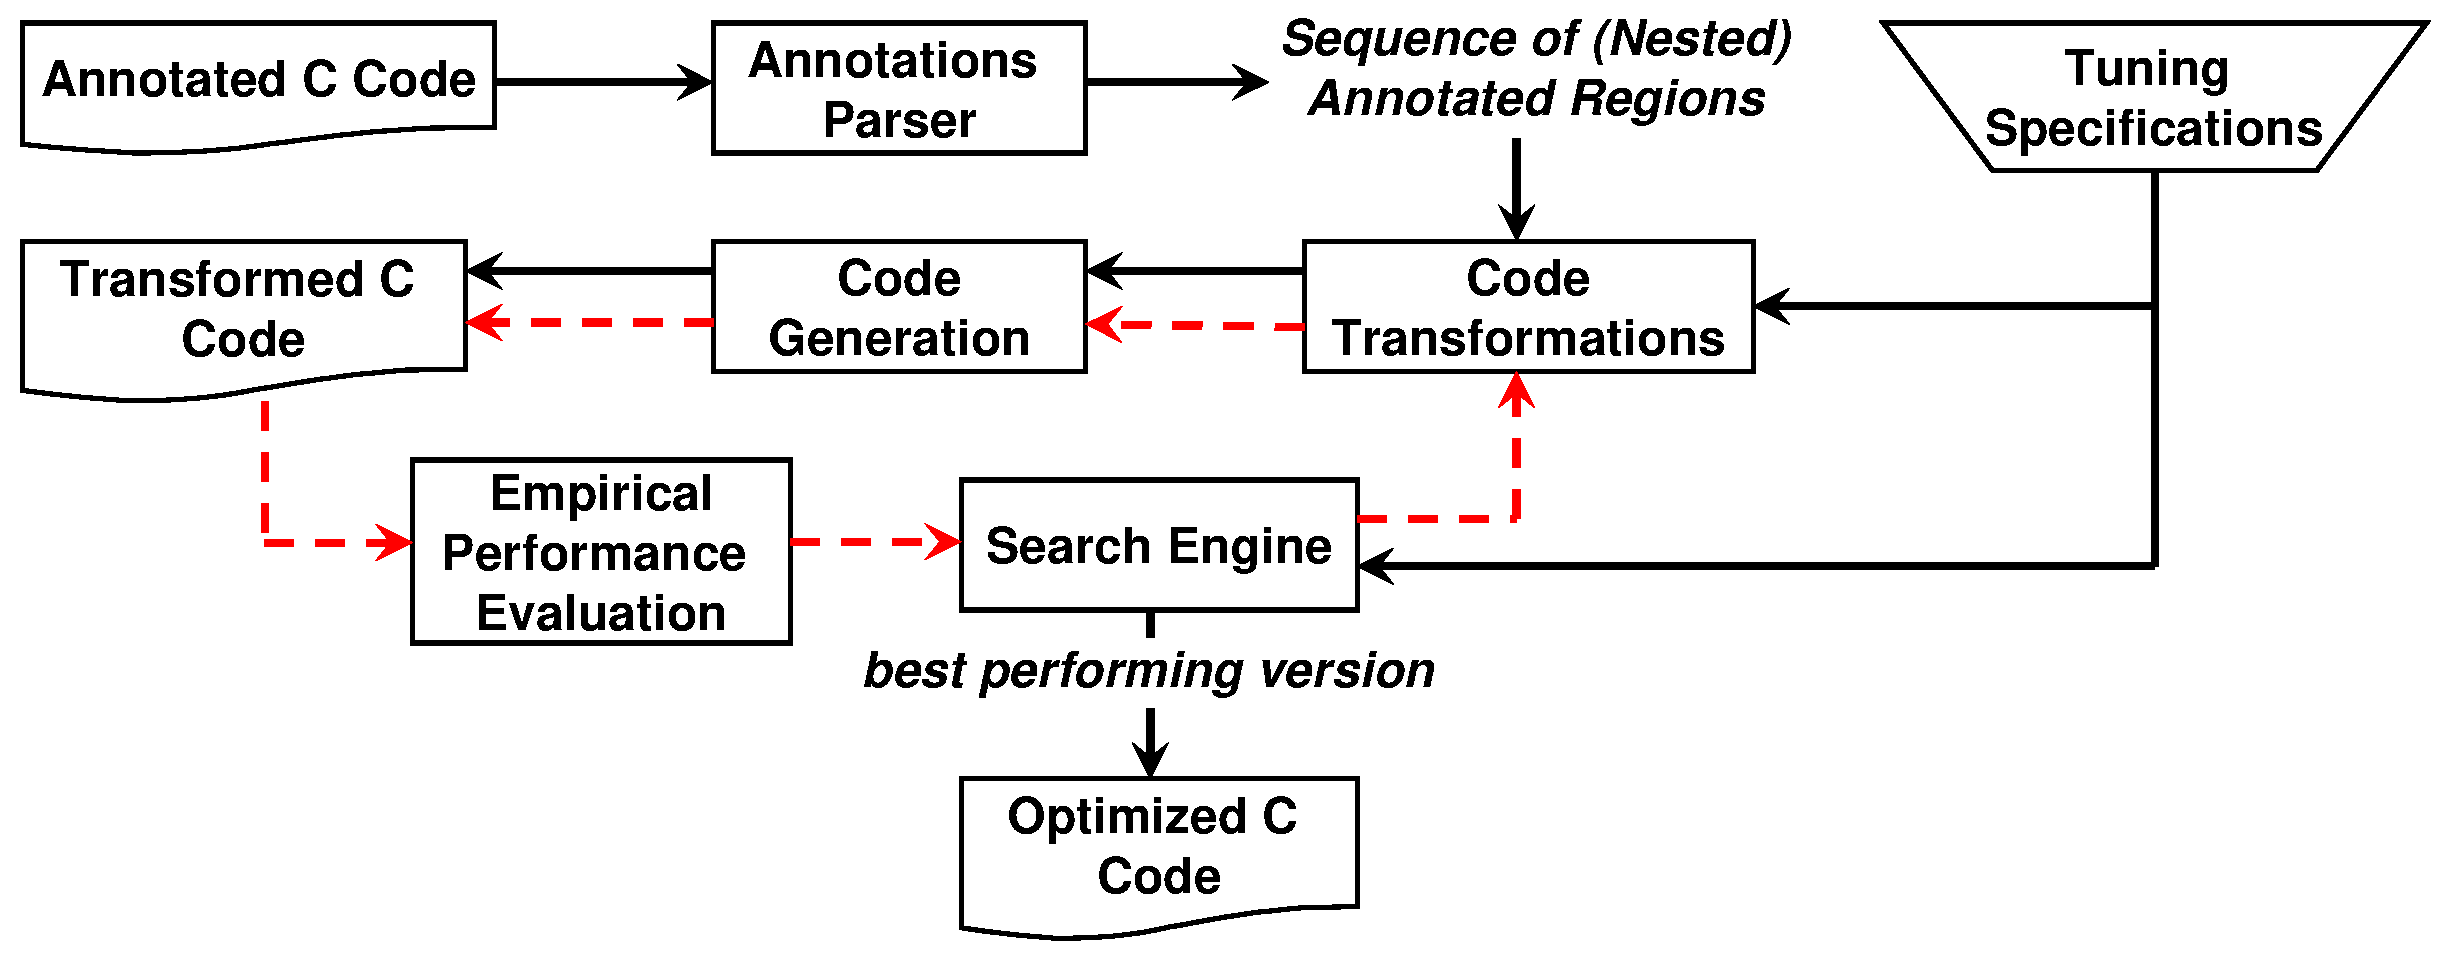
\includegraphics[width=0.6\textwidth]{figures/orio.eps}   
\end{center}
\caption{Overview of Orio's code generation and empirical tuning process.}  
\label{fig:orio}
\end{figure*}  

\begin{figure*}%[b]
\begin{center} 
\begin{tabular}{rrl} 
$<$annotation-region$>$ & ::= & $<$leader-annotation$>$ $<$annotation-body$>$ $<$trailer-annotation$>$\\ 
$<$leader-annotation$>$ & ::= & \texttt{/*@ begin} $<$module-name$>$ \texttt{(} $<$module-body$>$ \texttt{) @*/} \\
$<$trailer-annotation$>$ & ::= & \texttt{/*@ end @*/} \\
\end{tabular} 
\end{center}  
\caption{Annotation language grammar excerpt.}  
\label{fig:ann-lang}
\end{figure*}  

\section{Orio Design and Implementation}
\label{sec:implm}

Orio~\cite{OrioURL} is an empirical performance tuning system that takes
annotated C source code as input, generates many optimized code variants of
the annotated code, and empirically evaluates the performance of the
generated codes, ultimately selecting the best performing version to use for
production runs.

The Orio annotation approach differs from existing compiler- and
annotation-based systems in the following significant ways.
%
First, by not committing to a single general-purpose language, we can define 
annotation grammars that \emph{restrict} the original syntax, enabling more
effective performance transformations (e.g., disallowing pointer arithmetic
in a C-like annotation language); furthermore, it enables the definition of
new high-level languages which retain domain-specific
information that is normally lost in low-level C or Fortran
implementations. This in turn expands the range of possible performance-improving 
transformations.
%
Second, Orio was conceived and designed with the following requirements in mind: 
portability (which precludes extensive dependencies on external packages),
extensibility (new functionality must require little or no change to the
existing Orio implementation and interfaces that enable integration with
other source transformation tools must be defined), and automation
(ultimately Orio should provide tools that manage
\emph{all} the steps of the performance tuning process, automating each step 
as much as possible).
%
Finally, Orio is usable in real scientific applications without
requiring reimplementation. This ensures that the significant investments in
the development of complex scientific codes is leveraged to the greatest
extent possible.

Figure~\ref{fig:orio} contains a high-level graphical depiction of the code
generation and tuning process implemented in Orio.  Orio can be used to
improve performance by source-to-source transformations such as loop
unrolling, loop tiling, and loop permutation. The input to Orio is C code
containing structured comments that include a simplified expression of the
computation, as well as various performance-tuning directives. Orio scans the
marked-up input code and extracts all annotation regions. Each annotation
region is then processed by transformation modules. The code generator then
produces the final C code with various optimizations that correspond to the
specified annotations. Unlike compiler approaches, we do not implement a
full-blown C compiler; rather, we use a precompiler that parses only the
language-independent annotations.

Orio can also be used as an automatic performance tuning tool.  The code
transformation modules and code generator produce an optimized code version
for each distinct combination of performance parameter values. Then each
optimized code version is executed and its performance evaluated.  After
iteratively evaluating all code variants, the best-performing code is picked
as the final output of Orio. Because the search space of all possible
optimized code versions can be huge, a brute force search strategy is not
always feasible. Hence, Orio provides various search heuristics for reducing
the size of the search space and thus the empirical testing time.

%% BN: The info in the paragraph below is repeated later in the discussion.
%The tuning specifications written by users in the form of annotations
%are parsed and used by Orio to guide the transformations and the
%empirical tuning process. These specifications include essential
%information such as the used base compilers, the search strategy, the
%program transformation parameters, the input data sizes, etc.

\subsection{Annotation Language Syntax} 
\label{sec:ann-lang}

Orio annotations are embedded into the source code as structured C comments
that always start with \texttt{/*@} and end with \texttt{@*/}. For example,
the annotation \texttt{/*@ end @*/} is used to indicate the end of an
annotated code region. A simple grammar illustrating the basic syntax of Orio
annotations is depicted in Figure~\ref{fig:ann-lang}. An annotation region
consists of three main parts: leader annotation, annotation body, and trailer
annotation. The annotation body can be either empty or contain C code that
possibly includes other nested annotation regions. A leader annotation
contains the name of the code transformation module used to transform and
generate the annotated application code. A high-level description of the
computation and several performance hints are coded in the module body inside
the leader annotation. A trailer annotation, which has a fixed form (i.e.,
\texttt{/*@ end @*/}), closes an annotation region.

\subsection{Orio Input Example}
\label{sec:example}

Figure~\ref{fig:orio-example} shows a concrete annotation example that
empirically optimizes a C function for the Blue Gene/P
architecture. This is an instance of an AXPY operation, i.e., one that computes
$y=y+a_1 x_1+\cdots+a_n x_n$, where $a_1,\ldots,a_n$ are scalars and
$y,x_1,\ldots,x_n$ are one-dimensional arrays. The specific AXPY operation
considered in this example corresponds to $n=4$. The first annotation contains the
\texttt{BGP\_Align}\footnote{Architecture-specific annotations are simply ignored when the
code is being tuned on an architecture that doesn't support them.} directive,
which instructs Orio to dynamically load its memory-alignment optimization
module and then generate preprocessor directives, such as pragmas and calls
to memory alignment intrinsics, including a check for data alignment. The
main purpose of these alignment optimizations is to enable the use of the
dual floating-point unit (Double Hummer) of the Blue Gene/P, which requires
16-byte alignment. As discussed later in Section~\ref{sec:axpy4-results},
even these simple alignment optimizations can lead to potentially significant
performance improvements. This example also shows the use of Orio's loop
transformation module (named \texttt{Loop}) to optimize the AXPY-4 loop by
unrolling and generating OpenMP parallelization directives for exploiting
multicore parallelism. In addition to the simple source transformations in
this example, Orio also supports other optimizations, such as register
tiling and scalar replacement.

Whereas the \texttt{BGP\_Align} and \texttt{Loop} annotations in this example
guide the source-to-source transformations, the purpose of the
\texttt{PerfTuning} annotation is primarily to control the empirical
performance tuning process. Details of the tuning specifications for
optimizing the AXPY-4 code on Blue Gene/P are shown in the right-hand side of
Figure~\ref{fig:orio-example}.  The tuning specification contains data
required for building, initializing, and running experiments, including input
variable information, the search algorithm, performance counting technique,
performance parameters values, and execution environment details.  The tuning
specifications can be either integrated in the source code or defined in a
separate file, as in this example.

\begin{figure*}%[!t] 
\centering 
\begin{tabular}{cc} 
\begin{minipage}{.5\textwidth}  
\scriptsize
\begin{verbatim}  
 void axpy4(int N, double *y, 
  double a1, double *x1, double a2, double *x2, 
  double a3, double *x3, double a4, double *x4) {

  /*@ begin PerfTuning (
    import spec axpy4_tune_spec;
  ) @*/

  register int i;

  /*@ begin BGP_Align (x1[],x2[],x3[],x4[],y[]) @*/ 
  /*@ begin Loop ( 
   transform Unroll (ufactor=UF, parallelize=PAR)
   for (i=0; i<=N-1; i++) 
     y[i] += a1*x1[i]+a2*x2[i]+a3*x3[i]+a4*x4[i]; 
  ) @*/ 

  for (i=0; i<=N-1; i++) 
    y[i] += a1*x1[i]+a2*x2[i]+a3*x3[i]+a4*x4[i];

  /*@ end @*/ 
  /*@ end @*/
  /*@ end @*/
 }









\end{verbatim}  
\end{minipage}
&
\begin{minipage}{.5\textwidth}  
\scriptsize
\begin{verbatim}  
 spec axpy4_tune_spec {
  def build { 
   arg build_command = 
    'mpixlc_r -O3 -qstrict -qhot -qsmp=omp:noauto'; 
   arg batch_command = 
    'qsub -n 128 -t 20 --env "OMP_NUM_THREADS=4"'; 
   arg status_command = 'qstat';
   arg num_procs = 128; 
  } 
  def performance_counter { 
   arg method = 'basic timer';
   arg repetitions = 10000;
  } 
  def performance_params { 
   param UF[] = range(1,33);
   param PAR[] = [True,False]; 
  }
  def input_params { 
   param N[] = [10,100,1000,10**4,10**5,
                10**6,10**7]; 
  }
  def input_vars { 
   decl dynamic double y[N] = 0; 
   decl dynamic double x1[N] = random; 
   decl double a1 = random; 
   decl double a2 = random; 
   # ... ommitted ...
  } 
  def search { 
   arg algorithm = 'Exhaustive'; 
   arg time_limit = 20;
  }
 }
\end{verbatim}  
\end{minipage}
\\
\end{tabular}
\caption{Orio input example; annotated AXPY-4 source code (left) and tuning specification for the Blue Gene/P (right).}
\label{fig:orio-example}  
\end{figure*} 

\begin{figure*}%[!t] 
\centering 
\begin{tabular}{cc} 
\begin{minipage}{.5\textwidth}  
\scriptsize
\begin{verbatim}  
 /*@ begin Loop (
 transform UnrollJam(ufactor=Ui)
 for (i=0; i<=M-1; i++)
   transform UnrollJam(ufactor=Uj)
   for (j=0; j<=N-1; j++)
     transform UnrollJam(ufactor=Uk)   
     for (k=0; k<=O-1; k++)
       A[i][j] += B[i][k]*C[k][j];
 ) @*/
 for (i=0; i<=M-1; i++)
  for (j=0; j<=N-1; j++)
   for (k=0; k<=O-1; k++)
     A[i][j] += B[i][k]*C[k][j];
 /*@ end @*/
\end{verbatim}  
\end{minipage}
&
\begin{minipage}{.5\textwidth}  
\scriptsize
\begin{verbatim}  
 def performance_params {
   param Ui[] = range(1,33);
   param Uj[] = range(1,33);
   param Uk[] = range(1,33);
   constraint reg_capacity = Ui*Uj+Ui*Uk+Uk*Uj<=32;
 }

 def input_params {
   param M[] = [10,50,100,500,1000];
   param N[] = [10,50,100,500,1000];
   param O[] = [10,50,100,500,1000];
   constraint square_matrices = (M==N) and (N==O);
 }

\end{verbatim}  
\end{minipage}
\\
\end{tabular}
\caption{Example of specifying parameter constraints in Orio; annotated code for matrix-matrix multiplication (left) and constraint specification (right).}
\label{fig:par-constraint}  
\end{figure*} 

The annotated AXPY-4 code (left side of Figure~\ref{fig:orio-example}) uses two
performance parameters whose values are defined in the tuning specification:
the unroll factor (\texttt{UF})
% which signifies how many times the loop body will be
%replicated in the generated code.
and the boolean variable \texttt{PAR}, which is used to activate or
deactivate OpenMP parallelization. 
%Such boolean parameter is needed by Orio
%due to the following basis: when both the number of loop iterations and the
%total amount of computation in the loop body are small, parallelizing a loop
%using OpenMP can give poor performance because of the dominating overhead
%incurred from thread coordination and task scheduling. Therefore, based on a
%given vector size, Orio can determine at runtime whether it is beneficial to
%parallelize the loop.
These parameters are used by Orio to determine at runtime whether it is
beneficial to parallelize the loop, i.e., whether there is enough work per
thread to offset the OpenMP overhead or not.

Achieving the best performance for different input problem sizes may require
different tuning approaches; thus, the entire tuning process is
repeated for each specified problem size. In the AXPY-4 example, the search
space includes seven different input problem sizes (variable~\texttt{N}). 
%Orio repeats the tuning process for each problem size, resulting
%in the generation of seven final optimized codes.

\subsection{Annotation Parsing and Code Generation}

The Orio system consists of several optimization modules, each implemented as
a Python module. As mentioned earlier in Section~\ref{sec:example}, given the
module name in the leader annotation, Orio dynamically loads the
corresponding code transformation module and uses it for both annotation
parsing and code generation. If the pertinent module cannot be found in the
transformation modules directory, an error message is emitted and the tuning
process is terminated. This name-based dynamic loading provides flexibility
and easy extensibility without requiring detailed knowledge or modification
of the existing Orio software. Therefore, varied approaches to code
transformations ranging from low-level loop optimizations for cache
performance to composed linear algebra operations and new specialized
algorithms can easily be integrated into Orio.

%Taking as input the information supplied in both the annotation body
%and the module body, 
After parsing the annotation, each module performs a distinct optimization
transformation prior to generating the optimized code.  The transformation
module can either reuse an existing annotation parser or define new language
syntax and a corresponding parser component. 

%%BN: the details below are probably not essential for this paper
%In some cases, the annotation is seemingly redundant, containing a version of
%the computation that is very similar to the original code. 
%We took this
%approach for two reasons.  First, basing the transformation modules on the
%actual application code demands a full-fledged C compiler
%infrastructure. Requiring this complex compiler infrastructure to avoid a
%relatively small manual effort in creating annotations runs counter to our
%goal of creating the annotation system portable and easy to install and
%use. Second, requiring in effect a rewrite of the code to be optimized
%encourages simplification and enables the code optimization effort to start
%with a cleaner, rather than an already hand-tuned, version of the
%code. Moreover, we are investigating higher-level, domain-specific syntax for
%annotations, thus capturing semantics without imposing tuning constraints
%resulting from the use of the general-purpose C language. 
In some cases, the annotation is seemingly redundant, containing a version of
the computation that is very similar to the original code.  As mentioned
earlier, we took this approach so that the annotation language can be defined
in a way that enables more effective transformations (through restrictions or
high-level domain information).

Current optimizations supported by Orio span different types of code
transformations that are not provided by production compilers in some
cases. Available optimizations include simple loop unrolling, memory
alignment optimization, loop unroll/jamming, loop tiling, loop permutation,
scalar replacement, register tiling, loop-bound replacement, array copy
optimization, multicore parallelization (using OpenMP), and other
architecture-specific optimizations (e.g., generating calls to SIMD
intrinsics on Intel and Blue Gene/P architectures).

\subsection{Search Space Exploration and Evaluation}
\label{sec:search-space}

As briefly discussed earlier, our empirical tuning approach systematically
measures the performance costs of automatically-generated code variants in
order to find the most optimal available version. In the context of empirical
optimization, code variants are alternative, semantically equivalent,
implementations of the same computation. Each implementation variant is
associated with a collection of different optimization parameters that
correspond to source-to-source code transformations such as, for instance,
unroll factors, tile sizes, and loop permutation order. So, each coordinate
in the search space of empirical tuning problem represents a distinct
combination of performance parameter values. Both the dimension and the size
of the search space depend on the total number and the value ranges of used
performance parameters, respectively.

The conceptually straightforward approach to exploring the space of the
parameter values is to use an exhaustive search procedure that is guaranteed
to determine the optimal code version. Normally the size of the search space
is too large, making full coverage impractical.  Thus, in addition to
supporting exhaustive search, we have implemented several search heuristics.
The simplest search heuristic is a random search, which picks a random
coordinate in the search space at each step and then measures its
performance; random search is not guaranteed to return close-to-optimal results.
We have also developed two other search heuristics to effectively
narrow the search space for close-to-optimal performance, including a
heuristic based on the \textit{Nelder-Mead simplex}
method~\cite{Lagarias98simplex,Lewis00directsearch}, 
a popular non-derivative direct search method for optimization, and \textit{simulated
annealing}\cite{Kirkpatrick83optimizationby}.
%with the additional inclusion of
%a gradually-reduced ``temperature'' used to control the randomness of
%selecting the next move in the search space. 
%By default Orio uses exhaustive
%search, but users can set the search parameters in the tuning specification
%to use and configure one of the available heuristics.  
Similarly to the implementation of Orio's optimization modules, each search
technique is implemented as an independent Python module in Orio and is dynamically
loaded given only the algorithm's name as one of the fields in the tuning
specification.

%%BN: commenting for space
%The key idea of a basic simplex method
%is to construct a nondegenerate simplex (i.e., a convex hull of $n+1$ points,
%where $n$ is the dimension of the search space), and then obtain its
%associated function values to steer the search to the next move by replacing
%the worst vertex with a point reflected through the centroid of the remaining
%$n$ points. The simplex search is improved in the Nelder-Mead method by
%adding more moves, making the search more robust and faster to converge. \

%The exhaustive approach is chosen as the default space exploration
%method of Orio; however, users can switch to the other algorithms by
%manually indicating his preferred search strategy in the tuning
%specifications. Users can also specify terminating criteria of the
%chosen search strategy by providing numerical values to the search
%time limit and the maximum total number of search trials. Each time
%the search exceeds the specified time limit or the predetermined
%number of full search runs, we suspend the search and return the best
%implementation variant up to that point of time. Also, users can
%optionally adjust the search by altering the values of some
%algorithm-specific parameters in the tuning specifications. As an
%example, users can change four types of coefficients that the
%Nelder-Mead simplex method has: reflection, expansion, contraction,
%and shrinkage, in order to control the search convergence speed and
%the quality of the search outcome.

To improve the quality of the search result further, each search heuristic is
enhanced by applying a local search after the global search completes. The
local search compares the best performance with neighboring coordinates. If a
better coordinate is discovered, the local search continues recursively until
no further performance improvement is possible or a user-specified
termination criterion is met.

Further pruning of the search space is enabled through user-specified
constraints in the tuning specifications. We use loop the
unroll/jamming transformation to make the discussion more concrete. Loop
unroll/jamming~\cite{sarkar-unrolljam} (coupled with scalar replacement) is
mainly intended to increase data reuse at the register level. So, when
unroll/jamming is applied to multiple loops, the values of unroll factors
must be such that register locality is maximized while satisfying the
register capacity constraints to avoid unnecessary register
spills. Figure~\ref{fig:par-constraint} shows an example of analytically
enforcing register capacity constraints on matrix-matrix multiplication code
that is optimized with loop unroll/jamming, assuming 32
registers. \texttt{Ui}, \texttt{Uj}, \texttt{Uk} are unroll factors for loops
\texttt{i}, \texttt{j}, \texttt{k}, respectively. With the specified
parameter constraints, the search space of performance parameter values is
drastically trimmed down from 32,768 points (i.e., $32*32*32$) to only 65
points. This example also demonstrates that a set of constraints can also be
imposed on input parameters to decide what input problem sizes to consider.

Orio also supports parallel search when parallel resources are available,
e.g., when tuning on the Blue Gene/P. The parallel Orio driver concurrently
executes multiple independent code variants in the same parallel job. After
Orio submits a parallel job, each node in the target machine executes a
distinct generated code variant to collect the code performance. The
resulting performance results are collected and stored in a temporary file,
which is later processed by Orio to determine the best performing variant.
Figure~\ref{fig:orio-example} has an example of using parallel search by
specifying the number of nodes to use (per job) with the \texttt{num\_procs}
variable. The remaining fields used by the parallel search are the
\texttt{batch\_command} and the \texttt{status\_command} fields, which specify how Orio
should submit a parallel job and query its status, respectively.



\begin{figure*}[bt]
\begin{center}
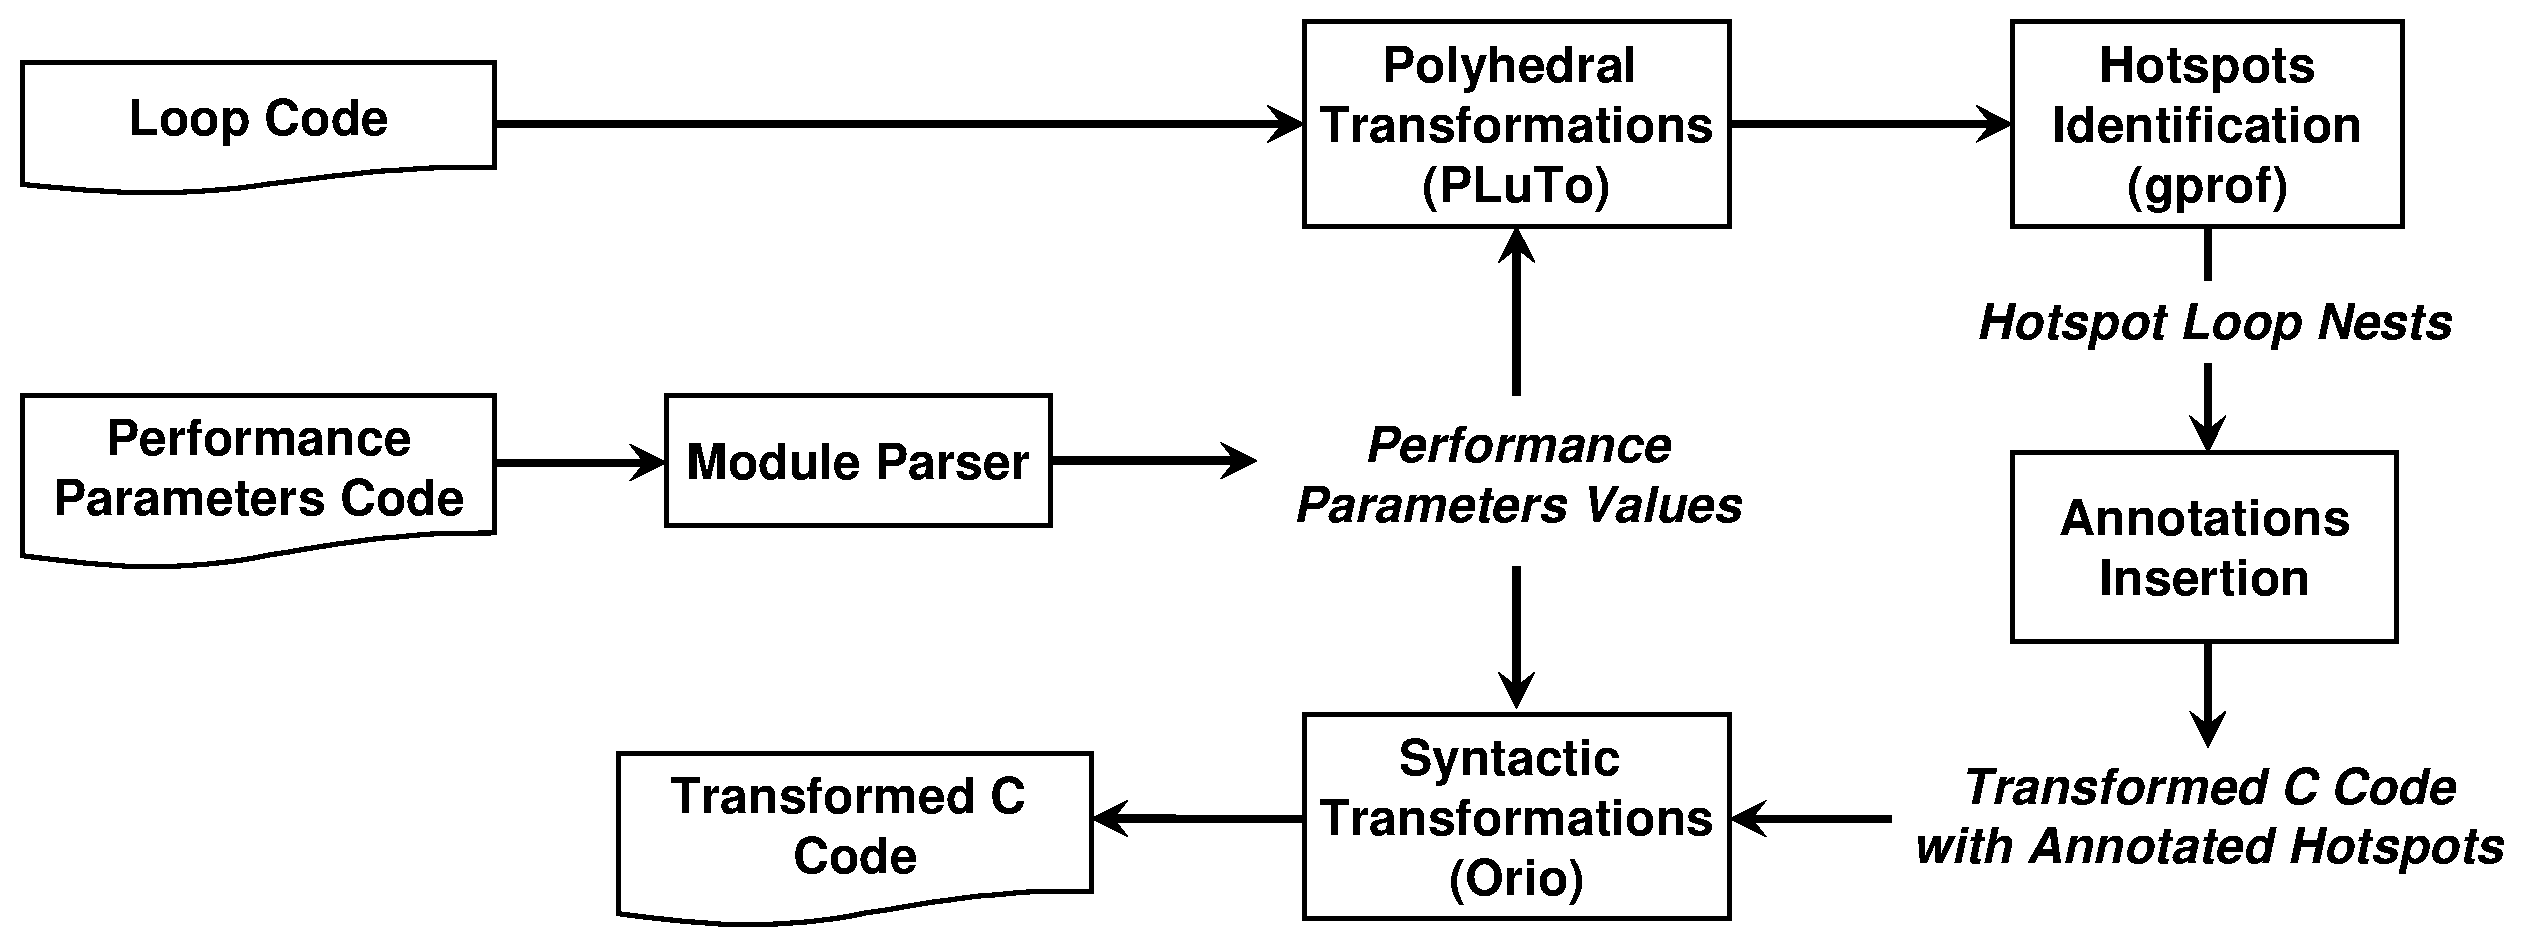
\includegraphics[width=0.6\textwidth]{figures/pluto-orio.eps}    
\end{center}   
\caption{Integration of Pluto into Orio's code transformation module.}
\label{fig:pluto-orio}
\end{figure*}  

\section{Pluto-Orio Integration}
\label{sec:integration}

A number of source-to-source transformation tools for performance
optimization exist. Using these tools to achieve (near) optimal performance
on different architectures, however, is still a nontrivial task that requires
significant architectural and compiler expertise. By combining code
transformation tools with an empirical tuning system, such as Orio, we can
reduce the amount of manual effort and automatically determine the
transformations that result in the best performance. We show in this section
how Orio has been extended with an external transformation program, called
Pluto~\cite{uday08pldi}. This integration also demonstrates the easy
extensibility of Orio and the ability to leverage other source transformation
approaches.

Pluto is a source-to-source automatic transformation tool aimed at optimizing
a sequence of nested loops for data locality and coarse-grained parallelism
simultaneously. Pluto employs a polyhedral model of arbitrary loop nests,
where the dynamic instance (iteration) of each statement is viewed as an
integer point in a well-defined space called the statement's polyhedron. This
statement representation and a precise characterization of data dependences
enable Pluto to construct mathematically correct complex loop
transformations. Pluto's polyhedral-based transformations result in improved
cache locality and loops parallelized for multicore architecture.

Figure~\ref{fig:pluto-orio} outlines the overall structure of the
Pluto-Orio integrated system, which is implemented as a new
optimization module in Orio. Initially, the transformation process
takes two kinds of input: the loop code to be optimized and the
optimization parameters code. The loop code is embedded in the
annotation body block, while the performance parameters code is
written in the module body block. A parser implemented inside
the new module parses the performance parameters code to extract their
values. The extracted values of the performance parameters include
tile sizes, unroll factors, loop order (permutation), as well as
several boolean values for triggering OpenMP parallelization, scalar
replacement, and auto-vectorization. Using these parameter values,
Pluto then performs polyhedral transformations (e.g., two-level tiling
and OpenMP parallelization) on the input loop code. The resulting
generated code is subsequently passed to the widely-available
profiling tool gprof~\cite{gprof} for hotspot detection. The
statistical information produced by gprof provides accurate locations
(line numbers) of the loop nests where the Pluto-generated code spends
most of its execution time. The identified hotspot loop nests are then
decorated with Orio's performance annotations for complementary
syntactic transformations (e.g., loop permutation, loop
unroll/jamming, scalar replacement, and explicit
auto-vectorization). Finally, Orio optimizes the annotated hotspots as
described in Section~\ref{sec:implm}.

Pluto also performs syntactic loop unroll/jam in a post-processing
pass. The target loops, however, are limited only to innermost loops with a
maximum depth of two (i.e., 1-D unrolling and 2-D unroll/jamming). So we
choose to use the loop unroll/jam transformation already available in
Orio, which is more flexible because it can be applied to loop nests of
depths larger than two.



At present Orio does not employ any data dependence analysis when performing
syntactic transformations. Therefore, there is no guarantee that the code
generated after syntactic transformations is correct. Because of this, the
tuning process using the integrated Pluto-Orio system is currently
semi-automatic---user involvement is required to decide whether it is safe
to apply a syntactic transformation on an identified hotspot.
%The user only needs
%to check the transformation legalities once, since the hotspots
%consistently have similar basic loop structure for different
%Pluto-generated code versions. Once all illegal syntactic
%transformations are known by the user, they must be switched off so
%that the tuning process can proceed fully automatic with no more human
%interventions.




\section{Experimental Results} 
\label{sec:results} 
 
In this section, we discuss the performance results of several experiments on
a multicore Intel Xeon workstation and a Blue Gene/P (both at Argonne). The
workstation has dual quad-core E5462 Xeon processors (8 cores total) running
at 2.8 GHz (1600 MHz FSB) with 32 KB L1 cache, 12 MB of L2 cache (6 MB shared
per core pair), and 2 GB of DDR2 FBDIMM RAM, running Linux kernel version
2.6.25 (x86-64). Each compute node of the Blue Gene/P is equipped with four
850MHz IBM PowerPC 450 processors with a dual floating-point unit and 2GB
total memory per node, private L1 (32 KB) and L2 (4 MB) caches, a shared L3
cache (8 MB), and running a proprietary lightweight operating system. We used
version 10.1 of the Intel and version 9.0 of the IBM XL C/C++ V9.0 compilers
on the Xeon and Blue Gene/P, respectively. Because of space considerations,
here we discuss a limited number of computational kernels; more performance
results for different computations are available at the Orio project
website~\cite{OrioURL}.

\subsection{Sequence of Linear Algebra Operations} 
\label{sec:axpy4-results}
 
In this experiment, we tuned the performance of the AXPY-4 operation (see
Figure~\ref{fig:orio-example}) on a single node of the Blue Gene/P machine
using the IBM xlc compiler.  We measured the performance for two scenarios:
using a single core per node and using all four cores. The results are shown
in Figures~\ref{fig:axpy4-bgp-seq} and~\ref{fig:axpy4-bgp-par},
respectively. The single-core scenario was compiled with the following options:
\texttt{-O3 -qstrict -qarch=450d -qtune=450 -qhot -qsmp=noauto};  the
multicore scenario differs in the use of \texttt{-qsmp=auto} for the non-Orio
versions. The parallel Orio version contains OpenMP parallelization
directives in the generated code, thus necessitating the use of the
\texttt{-qsmp=omp:noauto} compiler option. Included are performance numbers for four
code variants: a simple loop implementation without any library calls
(labeled ``Compiler-optimized''), two BLAS-based implementations that use
Goto BLAS~\cite{Goto:2006fk} and the ESSL~\cite{ESSL} libraries, and the
Orio-tuned version.

\begin{figure}[thb] 
\begin{center} 
  \subfigure[Sequential (single core)]{ 
  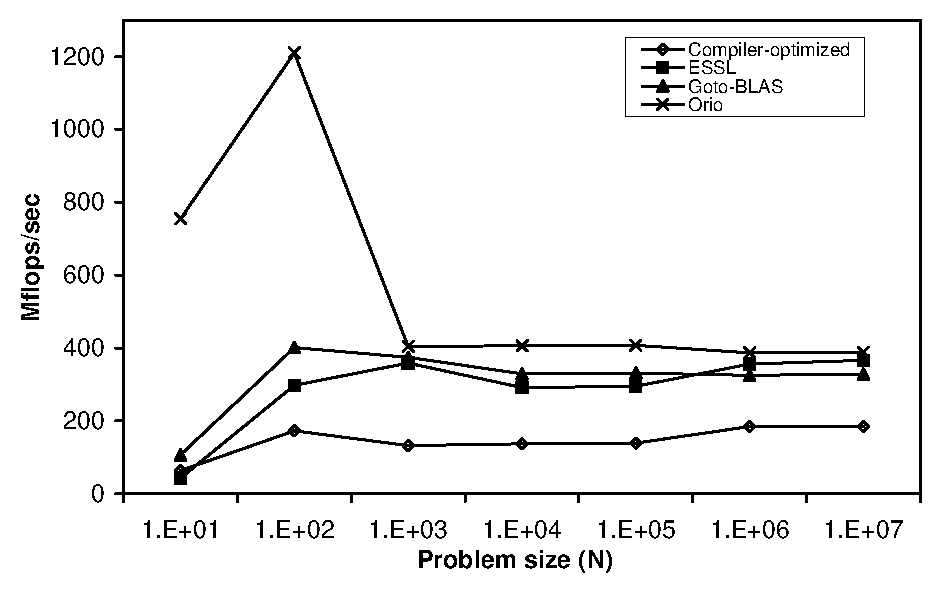
\includegraphics[width=.4\textwidth]{figures/axpy4_bgp/seq.eps}  
  \label{fig:axpy4-bgp-seq} 
  } 
  \subfigure[Parallel (four cores)]{ 
  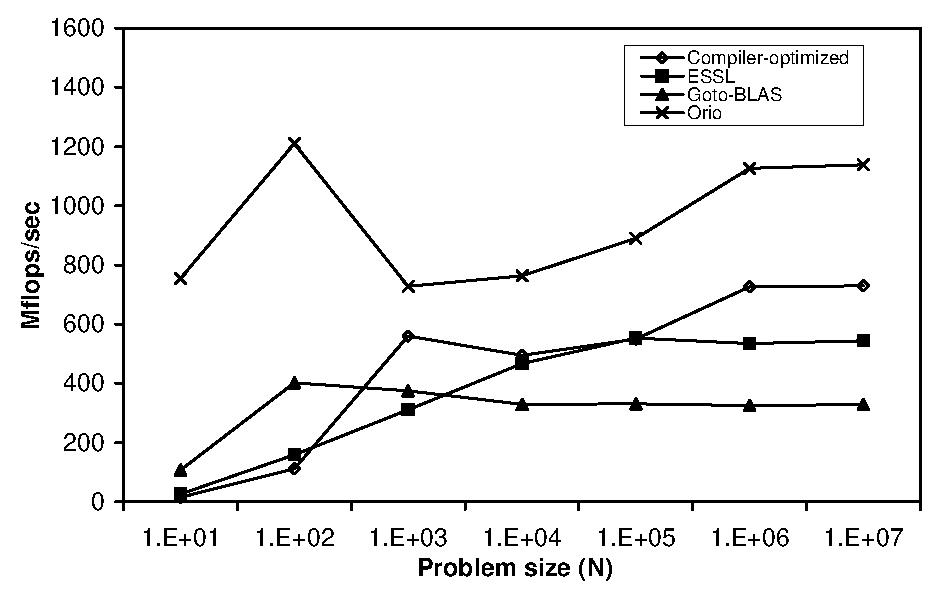
\includegraphics[width=.4\textwidth]{figures/axpy4_bgp/par.eps}  
  \label{fig:axpy4-bgp-par} 
  } 
\end{center}
\vspace{-.2in} 
\caption{Performance of AXPY-4 operations on the Blue Gene/P.} 
\label{fig:axpy4-bgp-results} 
\end{figure} 

The performance results shown in Figure~\ref{fig:axpy4-bgp-results} indicate
that the code tuned by Orio consistently outperforms the other three versions
for both the sequential and parallel cases. We observe that even for a simple
algebraic operation, such as the composed AXPY routines, the compiler alone
is unable to yield performance comparable to the empirically tuned
version. Moreover, implementations that rely on calls to multiple tuned
library routines (e.g., Goto BLAS and ESSL) suffer from loss of both spatial
and temporal localities, resulting in inferior memory performance.
%The sequential BLAS-based implementation perform better than the
%sequential single loop implementation. while for the parallel case, the 
%simple loop implementation is more efficient than the BLAS codes.

\subsection{Sparse Matrix Computations} 

In this section we examine the effectiveness of Orio in optimizing key
computations in PETSc~\cite{petsc-user-ref}, a toolkit for the parallel
numerical solution of partial differential equations, by empirically tuning
one of its heavily used kernels, sparse matrix-vector multiplication
(SpMV). SpMV dominates the performance of various scientific applications;
yet, traditional implementations of sparse kernels exhibit relatively poor
performance because of the use of indirect addressing for accessing the
matrix data elements.
%In
%order to attain higher performance, SpMV requires selecting a compact data
%structure and code transformations that best exploit properties of both the
%sparse matrix and the underlying architecture. Hence, the need for
%optimization and runtime tuning is a big distinction from the dense
%matrix-vector multiplication.

The SpMV operation computes $\forall_{A_{i,j}} \neq 0:y_{i}
\leftarrow y_{i} + A_{i,j} \cdot x_{j}$, where $A$ is a sparse matrix,
and $x$, $y$ are dense vectors. Each element of $A$ is used precisely once
and element reuse is only possible for $x$ and $y$. Thus, to optimize SpMV,
one should use compact data structures for $A$ and try to maximize temporal
reuse of $x$ and $y$. One of the most commonly used data structures for
storing a sparse matrix is compressed sparse row (CSR) storage,
%~\cite{vuduc-thesis} 
illustrated in Figure~\ref{fig:spmv}(a). Elements in each row of $A$ are
packed together in a dense array, \texttt{Aval}, and a corresponding array of
integers \texttt{Aind} stores the column indices. The \texttt{Aptr} array
designates where each sparse row begins in \texttt{Aval} and
\texttt{Aind}. An implementation of SpMV using CSR storage is
shown in Figure~\ref{fig:spmv}(b).

\begin{figure}[tb]
\centering
\vspace{-.2in}
\begin{tabular}{cc}
\begin{minipage}[b]{.5\textwidth}
\centering
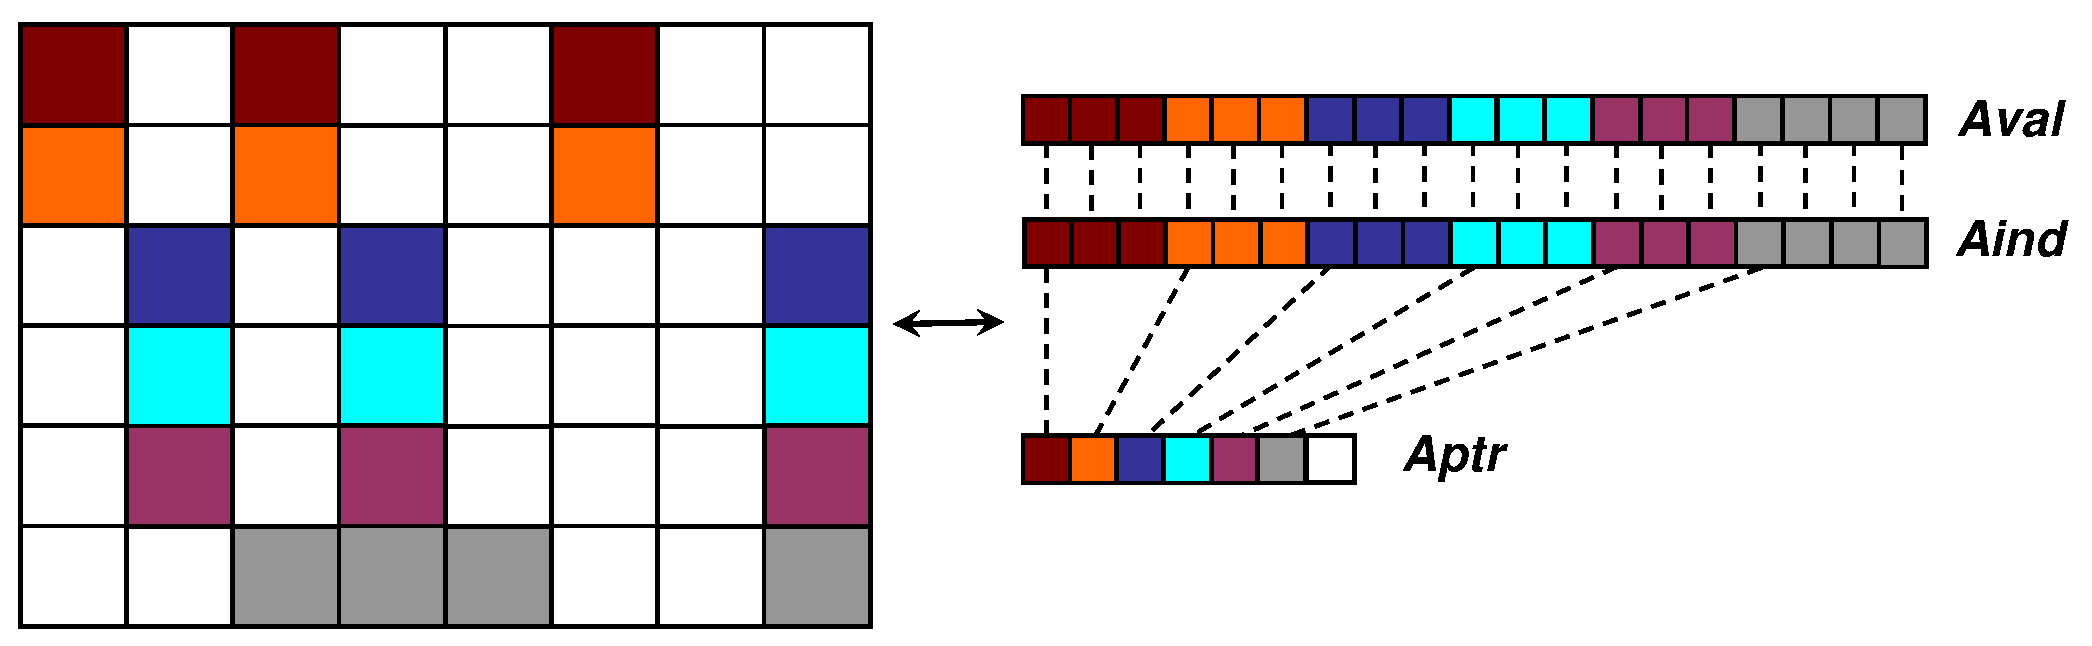
\includegraphics[width=.8\textwidth]{figures/spmv.eps}  
\end{minipage}
&
\begin{minipage}[b]{.5\textwidth}
\scriptsize
\begin{verbatim}
for (i=0; i<num_rows; i++)
  for (j=Aptr[i]; j<Aptr[i+1]; j++)
    y[i] += Aval[j]*x[Aind[j]];


\end{verbatim}
\end{minipage}\\
(a) & (b)\\
\end{tabular}
\vspace{-.2in}
\caption{(a) Compressed sparse row (CSR) format (b) Basic implementation of CSR-based SpMV.}
\label{fig:spmv}
%\vspace{.2in}
\end{figure}

PETSc's implementation of SpMV used in this experiment exploits matrix
structure by using \textit{inodes}, which represent rows with identical
nonzero structure.  PETSc detects inodes automatically in arbitrary sparse
matrices. For example, the sparse matrix shown in Figure~\ref{fig:spmv}(a)
contains three inodes. The first inode is of size two because it holds two
adjacent rows (i.e., the first and the second rows) with the same nonzero
structure. The second inode contains three consecutive rows with identical
nonzero structure, while the last inode only has a single row. Knowing the
properties of each inode at runtime enables maximum reuse of vector $x$ since
multiple elements of $x$ can be loaded and used exactly once for all rows in
the same inode structure. To accomplish this, one must use a
register-blocking transformation. To optimize the inode-based SpMV routine,
we incorporated a new transformation module inside Orio that implements
various optimization strategies including register blocking, SIMDization,
memory alignment optimization, loop-control optimization, accumulator
expansion, and thread-level parallelization (with OpenMP). We then used Orio
to automatically select the best version of the optimized inode SpMV. Only
the outer loop which iterates over inodes was parallelized by using OpenMP.

To evaluate the performance of the tuned SpMV routine, we conducted the
experiment using a 2-D driven cavity flow simulation
application~\cite{coff:kell:keye} (SNES ex27 in PETSc), on both the Xeon and
Blue Gene/P. The ``Compiler-optimized'' label is used as a base case that
represents the performance of the naive implementation of SpMV (shown in
Figure~\ref{fig:spmv}(b)) optimized by the native compiler. We also tested
the performance of the hand-tuned (by PETSc developers) SpMV code, which is
included in PETSc releases.

Figure~\ref{fig:ex27-cookie-results} shows the performance results on the
Intel Xeon. The problem size is the number of grid points in the $x$ and $y$
directions, not the size of the sparse input matrix. The matrix dimension is
based the grid size and the number of field components computed for each grid
point, for example, an $8 \times 8$ problem involves sparse matrices of
dimension 900 with 17,040 nonzero entries. In this experiment, we ran in
three different multicore modes: SMP (one MPI process, eight
threads/process), dual (four MPI processes, two threads/process), and virtual
node or VN (eight MPI processes, one thread/process). The code tuned by Orio
consistently outperforms the alternatives. Furthermore, the performance of
the hand-tuned code is almost equivalent to that of the icc-optimized simple
code. Performance differences between the Orio version and the hand-tuned
version become more significant as more threads per process are employed to
facilitate OpenMP parallelization. The SMP and VN results show that
optimizations using loop-level parallelism (through OpenMP) achieve much
better performance than using MPI coarse-grained parallelism.
%Moreover, for the multithread cases, tuning using Orio determined that
%the performance benefit of SIMDization is more significant than that of
%thread-level parallelization only when the problem sizes are small. The
%reason for this is due to the overhead introduced by OpenMP from coordinating
%its threads across processors.
%So, each optimized
%code for the many-thread cases comprises two distinct tuned codes to handle
\begin{figure} [ht]
\begin{center} 
  \subfigure[SMP: $p=1$, $t/p=8$]{
  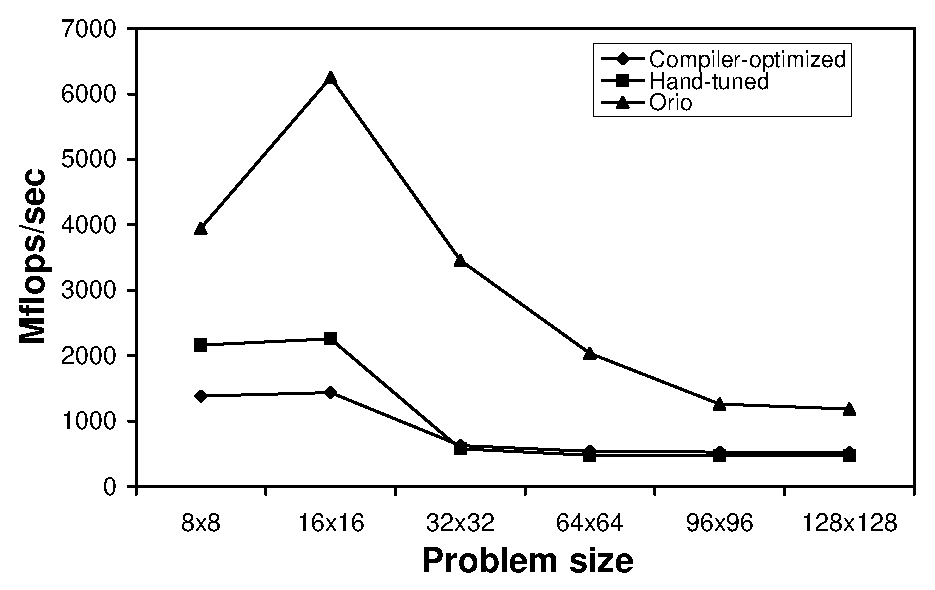
\includegraphics[width=.3\textwidth]{figures/ex27_cookie/smp.eps}
  \label{fig:ex27-cookie-smp} } \subfigure[Dual: $p=4$, $t/p=2$]{
  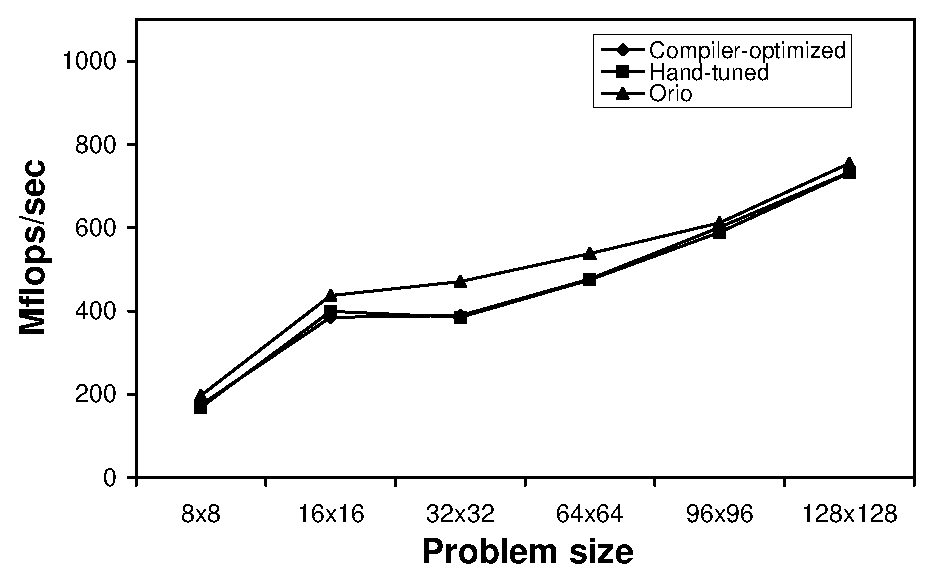
\includegraphics[width=.3\textwidth]{figures/ex27_cookie/dual.eps}
  \label{fig:ex27-cookie-dual} } \subfigure[VN: $p=8$, $t/p=1$]{
  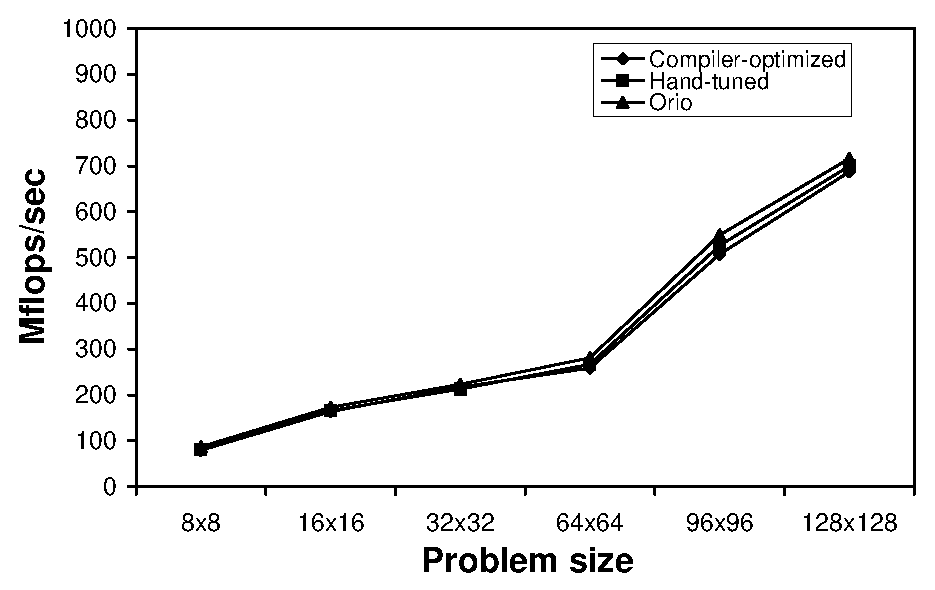
\includegraphics[width=.3\textwidth]{figures/ex27_cookie/vn.eps}
  \label{fig:ex27-cookie-vn} }
\end{center}
\vspace{-.2in} 
\caption{Performance of inode SpMV on eight-core Intel machine; $p$ is the number of processes, and $t/p$ is the threads per process.} 
\label{fig:ex27-cookie-results} 
\end{figure} 

The Blue Gene/P results in Figure~\ref{fig:ex27-bgp-results1} again show
%Blue Gene/P was done for a varied number of nodes (i.e., 1, 8, and 32)
%and the same three different parallel modes as before (i.e., SMP,
%dual, and VN). 
that empirical optimization using Orio produces the best performance for
all cases. 
%outperforming both the hand-tuned and the xlc-optimized codes. 
On this architecture, the performance gap between the xlc-optimized and the
hand-tuned codes is now larger than in the Intel experiment. Similarly, by
exploiting thread-level parallelism, the Orio-optimized code performs better
than the hand-tuned version when the number of threads per process increases
and the number of nodes decreases. For the single-thread cases (VN mode),
thread-level parallelism is not exploited; nevertheless, the Orio version
still performs better than the other two alternatives.
%This validates the
%effectiveness of Orio in empirically tuning sequential codes.

\begin{figure} [htb]
\begin{center} 
  \subfigure[1 node, SMP mode]{ 
  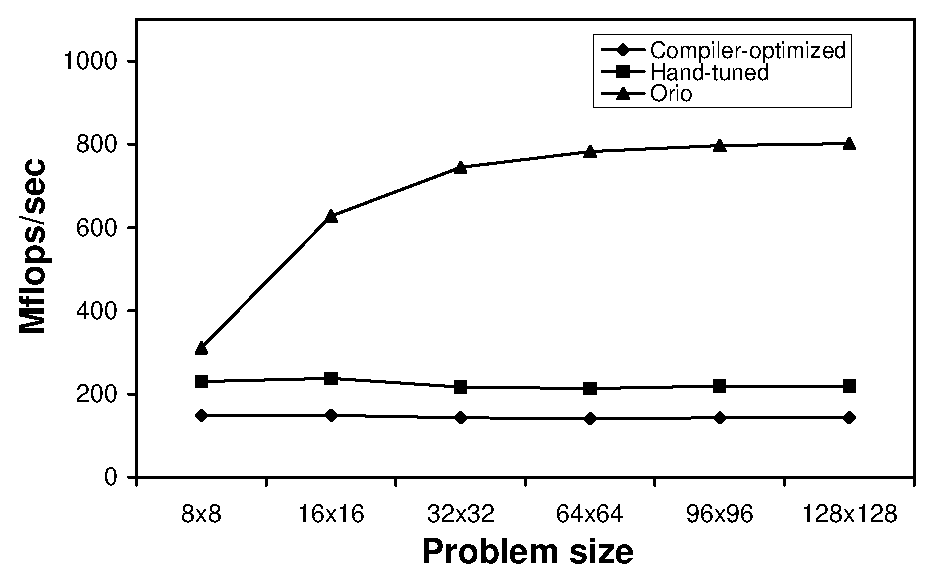
\includegraphics[width=.3\textwidth]{figures/ex27_bgp/n1_smp.eps}  
  \label{fig:ex27-bgp-smp-n1} 
  } 
  \subfigure[1 node, Dual mode]{ 
  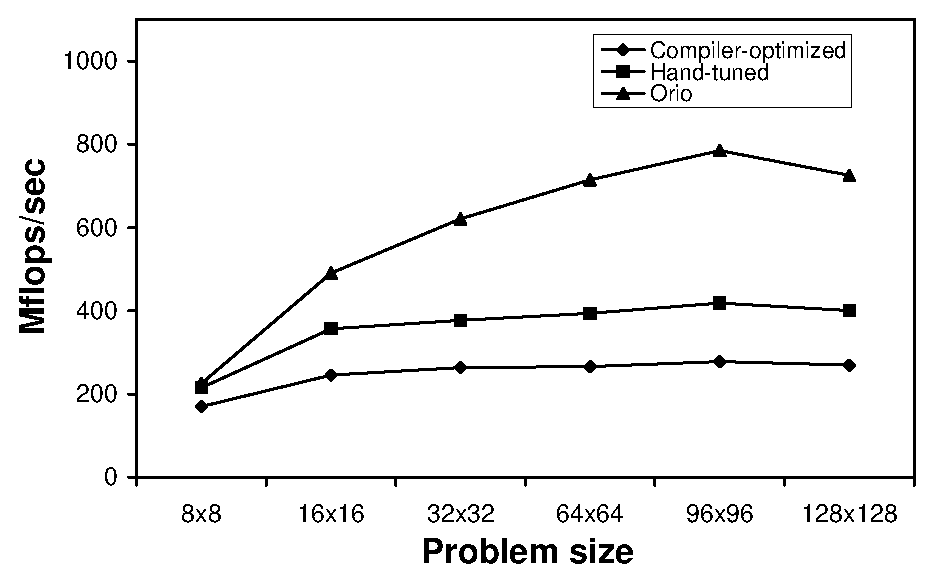
\includegraphics[width=.3\textwidth]{figures/ex27_bgp/n1_dual.eps}  
  \label{fig:ex27-bgp-dual-n1} 
  } 
  \subfigure[1 node, VN mode]{ 
  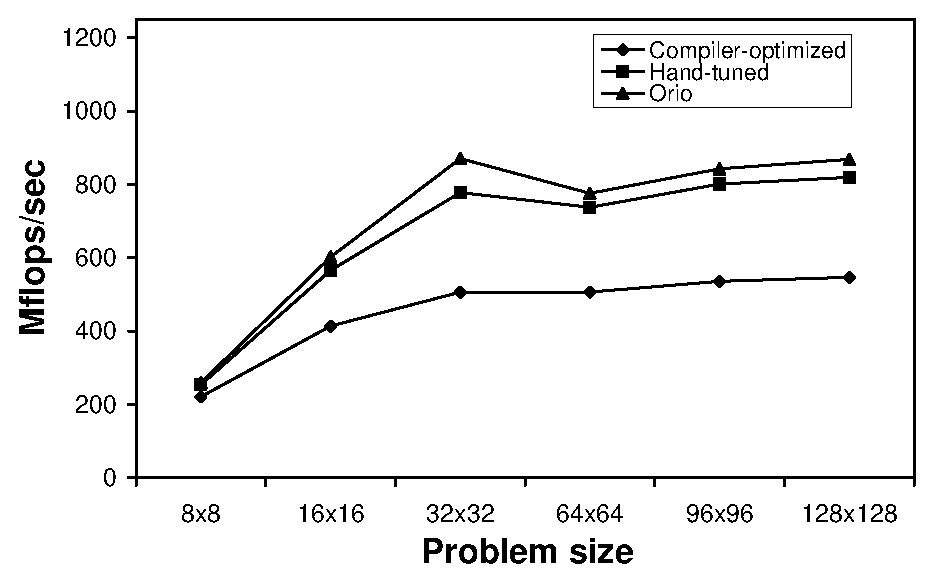
\includegraphics[width=.3\textwidth]{figures/ex27_bgp/n1_vn.eps}  
  \label{fig:ex27-bgp-vn-n1} 
  } 
  \subfigure[8 nodes, SMP mode]{ 
  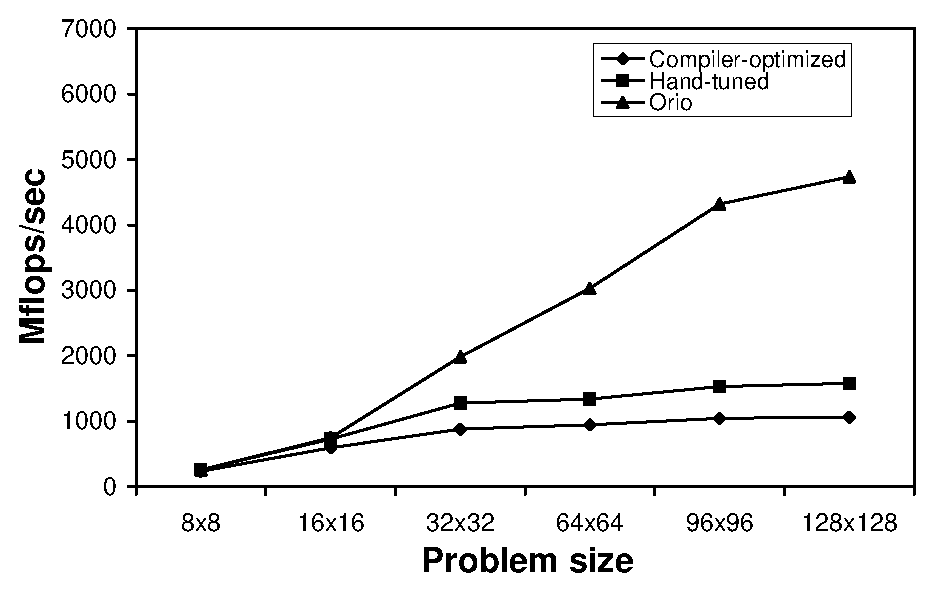
\includegraphics[width=.3\textwidth]{figures/ex27_bgp/n8_smp.eps}  
  \label{fig:ex27-bgp-smp-n8} 
  } 
  \subfigure[8 nodes, Dual mode]{ 
  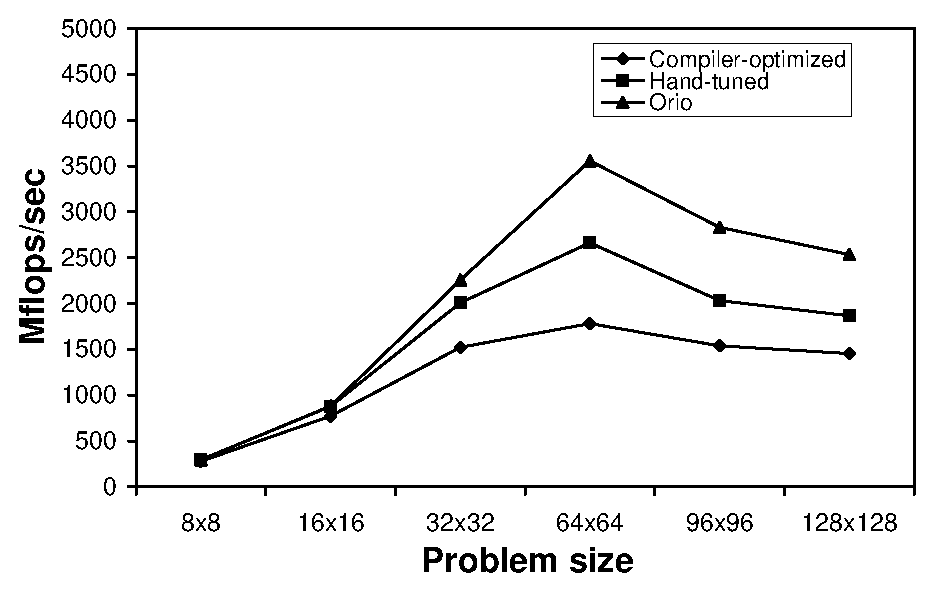
\includegraphics[width=.3\textwidth]{figures/ex27_bgp/n8_dual.eps}  
  \label{fig:ex27-bgp-dual-n8} 
  } 
  \subfigure[8 nodes, VN mode]{ 
  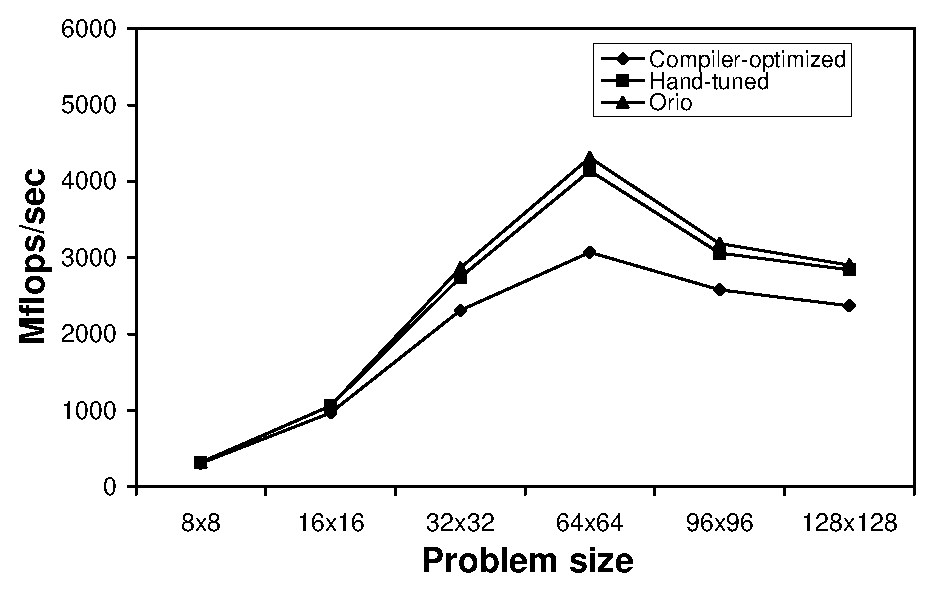
\includegraphics[width=.3\textwidth]{figures/ex27_bgp/n8_vn.eps}  
  \label{fig:ex27-bgp-vn-n8} 
  } 
%  \subfigure[32 nodes, SMP mode]{ 
%  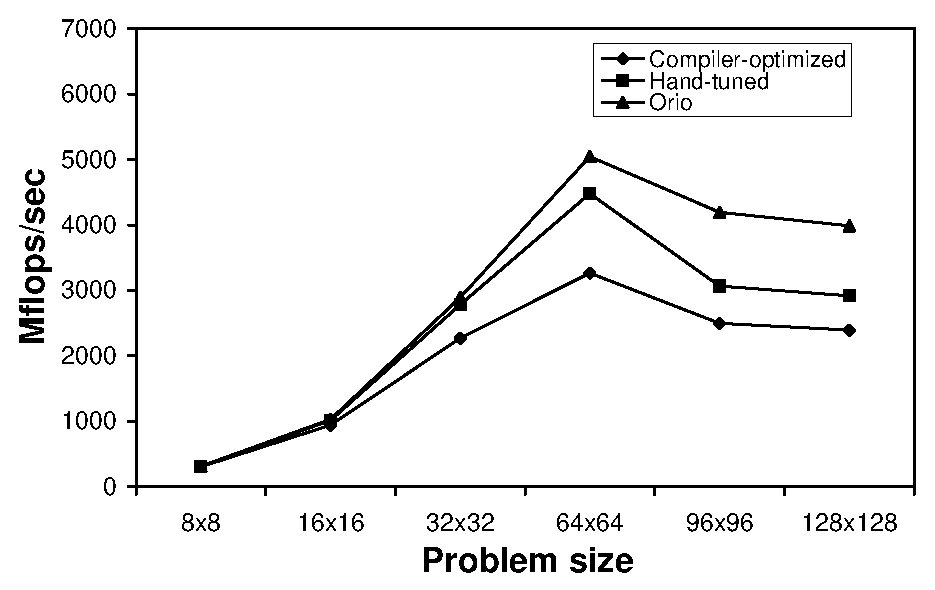
\includegraphics[width=.3\textwidth]{figures/ex27_bgp/n32_smp.eps}  
%  \label{fig:ex27-bgp-smp-n32} 
%  } 
%  \subfigure[32 nodes, Dual mode]{ 
%  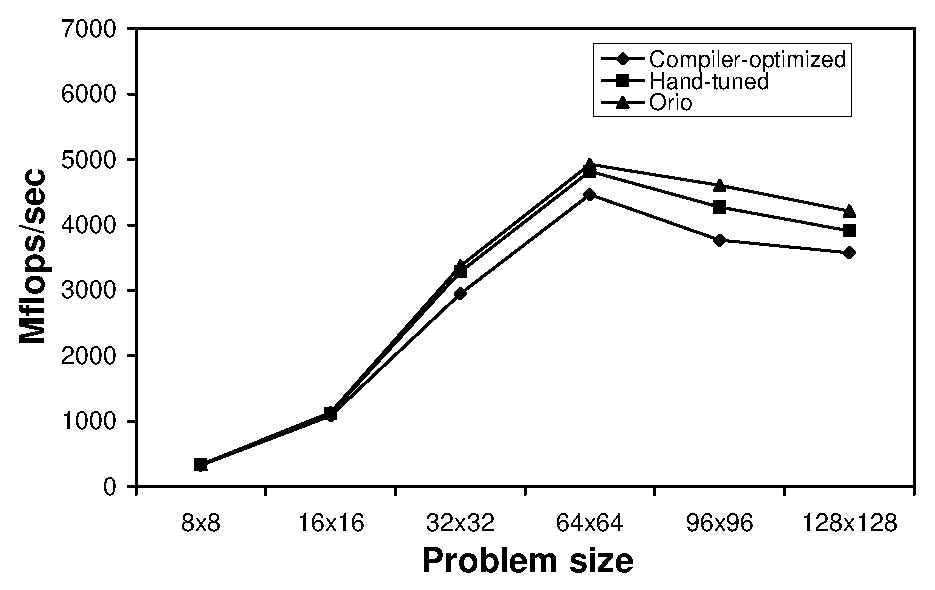
\includegraphics[width=.3\textwidth]{figures/ex27_bgp/n32_dual.eps}  
%  \label{fig:ex27-bgp-dual-n32} 
%  } 
%  \subfigure[32 nodes, VN mode]{ 
%  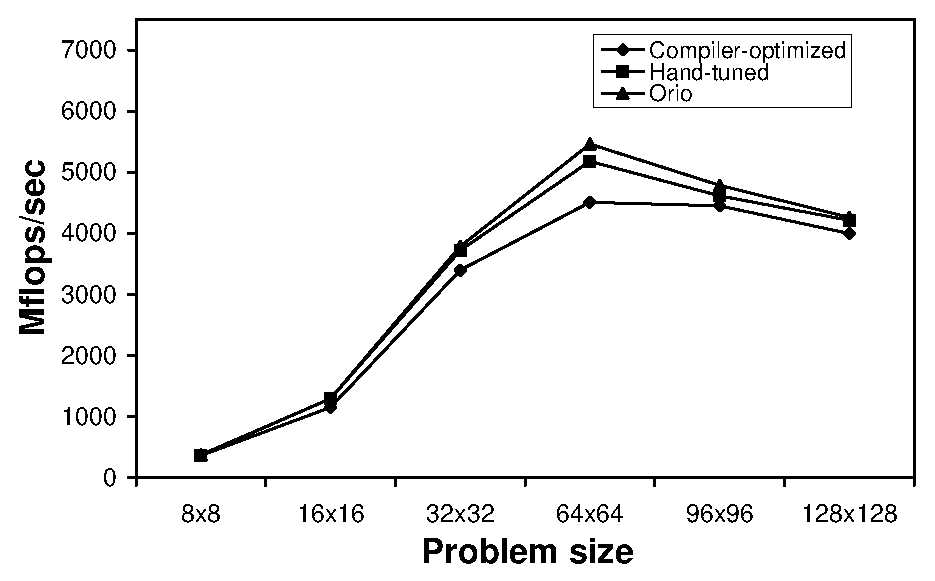
\includegraphics[width=.3\textwidth]{figures/ex27_bgp/n32_vn.eps}  
%  \label{fig:ex27-bgp-vn-n32} 
%  } 
\end{center}
\vspace{-.2in} 
\caption{Performance of inode SpMV on Blue Gene/P for 1, 8, and 32 nodes.} 
\label{fig:ex27-bgp-results1} 
\end{figure} 

\comment{
\begin{figure} 
\begin{center} 
  \subfigure[32x32, SMP mode]{ 
  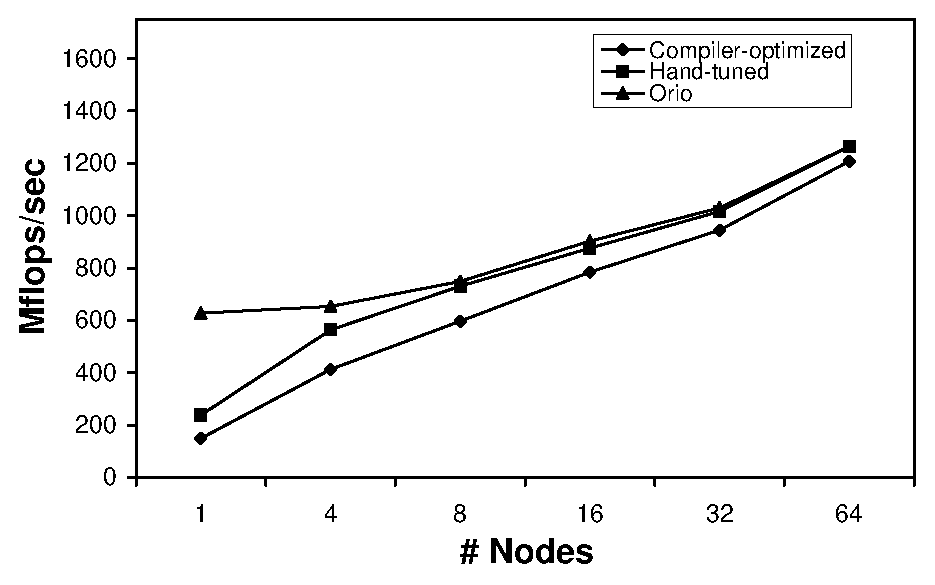
\includegraphics[width=.3\textwidth]{figures/ex27_bgp/s32_smp.eps}  
  \label{fig:ex27-bgp-smp-32x32} 
  } 
  \subfigure[32x32, Dual mode]{ 
  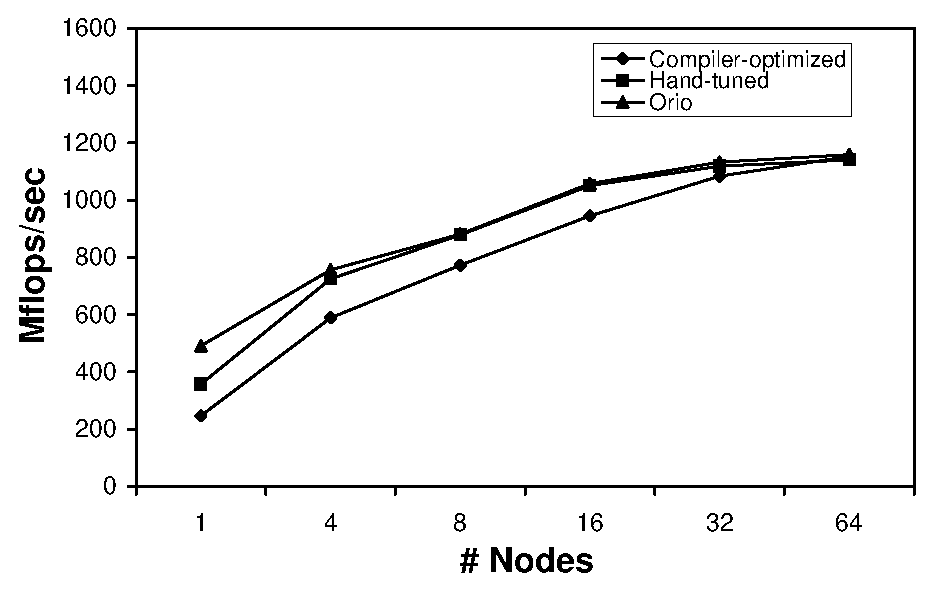
\includegraphics[width=.3\textwidth]{figures/ex27_bgp/s32_dual.eps}  
  \label{fig:ex27-bgp-dual-32x32} 
  } 
  \subfigure[32x32, VN mode]{ 
  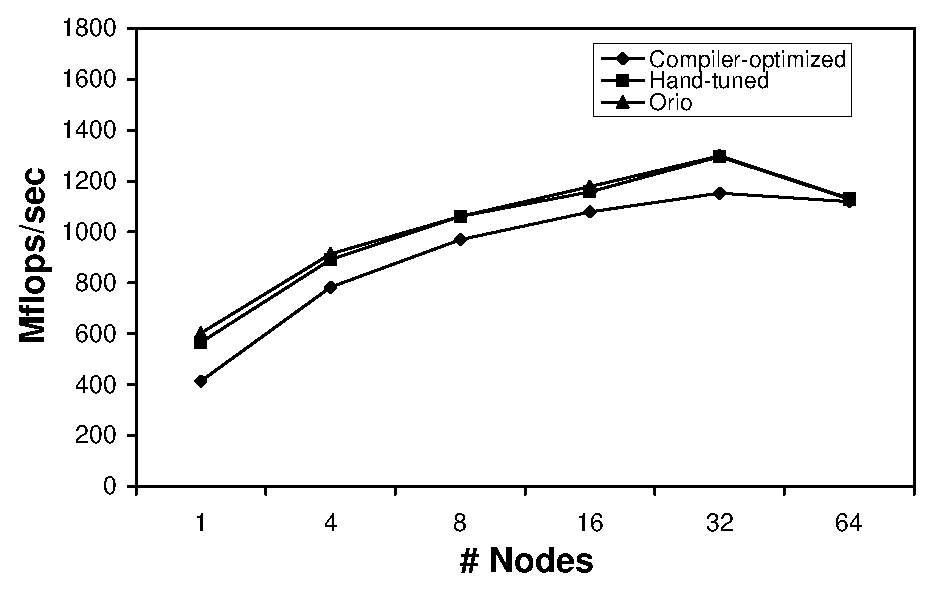
\includegraphics[width=.3\textwidth]{figures/ex27_bgp/s32_vn.eps}  
  \label{fig:ex27-bgp-vn-32x32} 
  } 
  \subfigure[64x64, SMP mode]{ 
  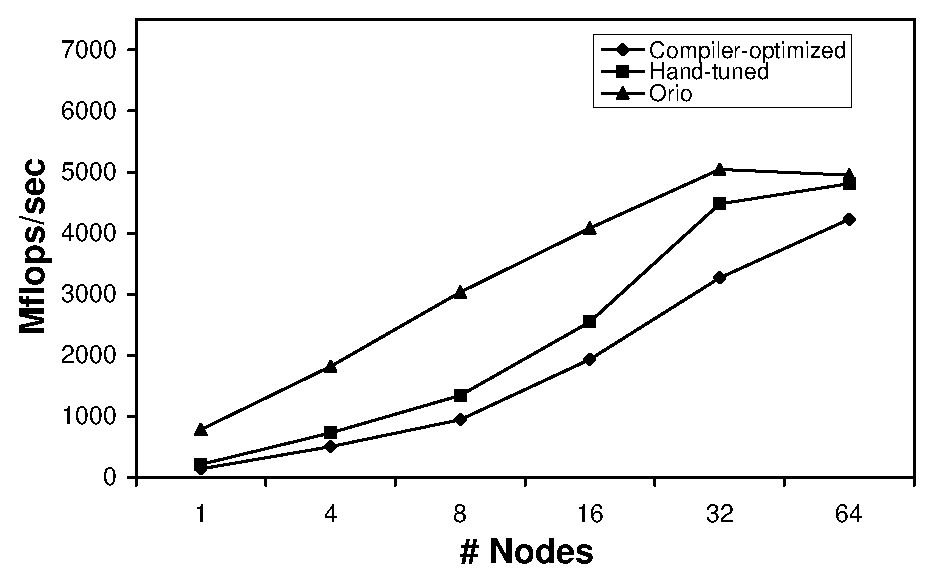
\includegraphics[width=.3\textwidth]{figures/ex27_bgp/s64_smp.eps}  
  \label{fig:ex27-bgp-smp-64x64} 
  } 
  \subfigure[64x64, Dual mode]{ 
  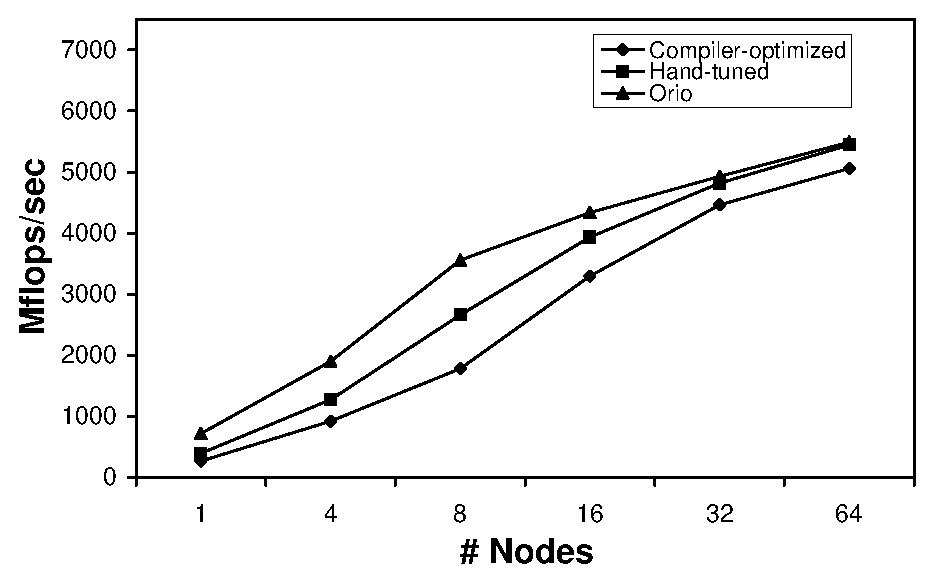
\includegraphics[width=.3\textwidth]{figures/ex27_bgp/s64_dual.eps}  
  \label{fig:ex27-bgp-dual-64x64} 
  } 
  \subfigure[64x64, VN mode]{ 
  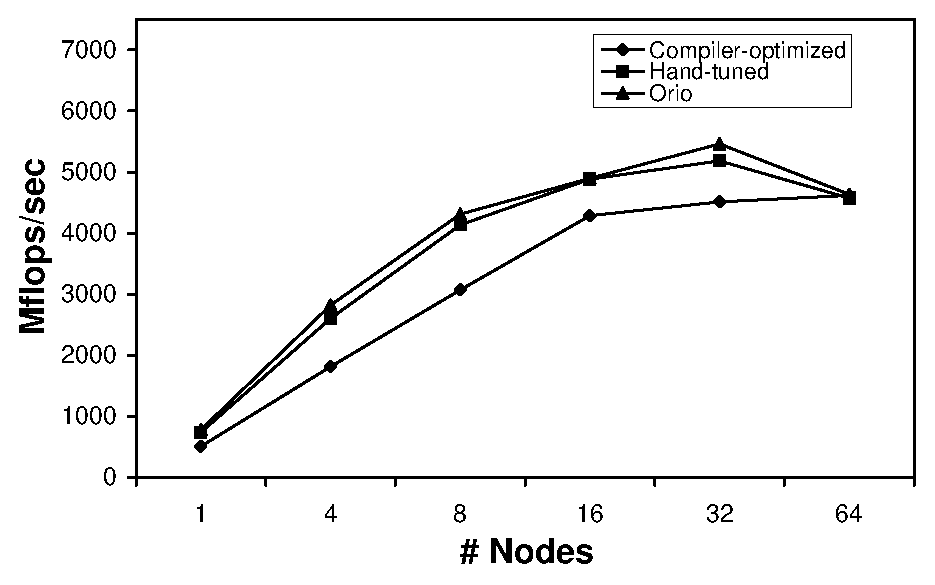
\includegraphics[width=.3\textwidth]{figures/ex27_bgp/s64_vn.eps}  
  \label{fig:ex27-bgp-vn-64x64} 
  } 
  \subfigure[128x128, SMP mode]{ 
  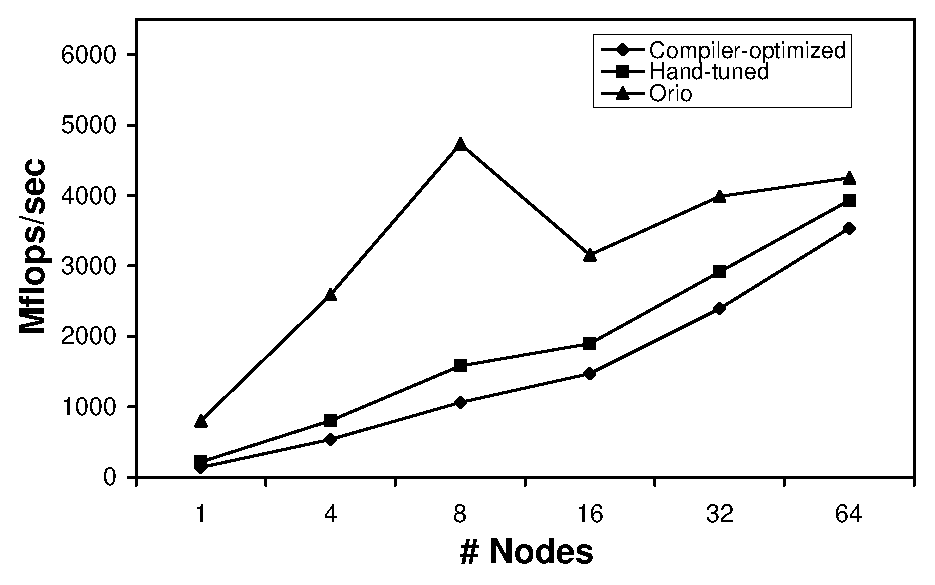
\includegraphics[width=.3\textwidth]{figures/ex27_bgp/s128_smp.eps}  
  \label{fig:ex27-bgp-smp-128x128} 
  } 
  \subfigure[128x128, Dual mode]{ 
  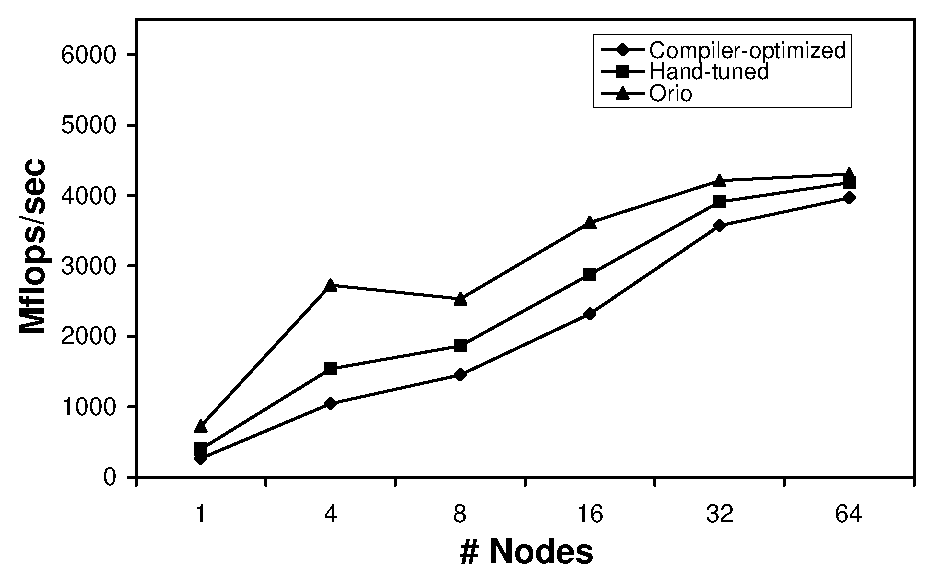
\includegraphics[width=.3\textwidth]{figures/ex27_bgp/s128_dual.eps}  
  \label{fig:ex27-bgp-dual-128x128} 
  } 
  \subfigure[128x128, VN mode]{ 
  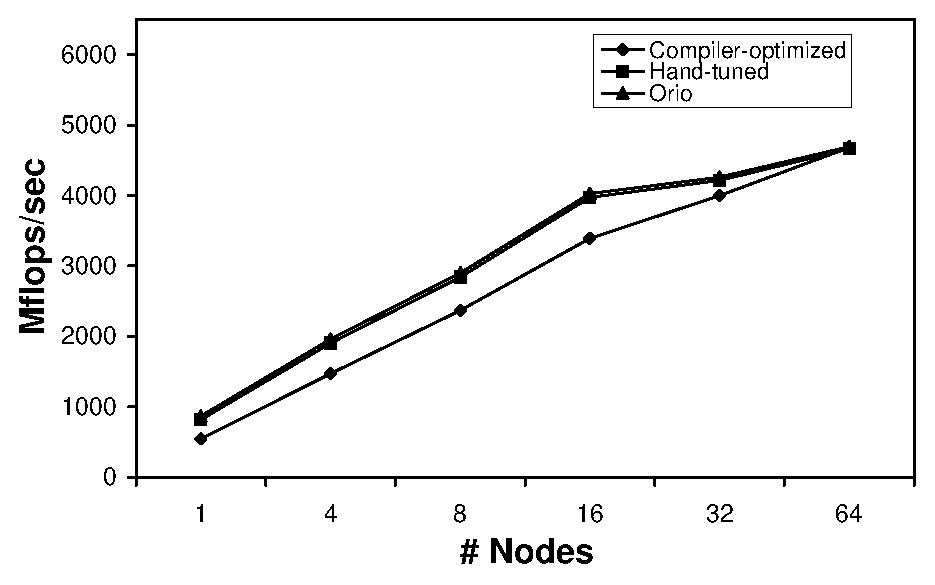
\includegraphics[width=.3\textwidth]{figures/ex27_bgp/s128_vn.eps}  
  \label{fig:ex27-bgp-vn-128x128} 
  } 
\end{center}
\vspace{-.2in}
\caption{Performance of inode SpMV on Blue Gene/P for problem sizes 32x32, 64x64, and 128x128.} 
\label{fig:ex27-bgp-results2} 
\end{figure} 
}

\subsection{Evaluation of the PLuTo-Orio Integrated System} 

This section discusses the performance evaluation of the integrated
PLuTo-Orio system (discussed in Section~\ref{sec:integration}) on the
multicore Intel Xeon by using a number of application kernels that are
nontrivial to optimize and parallelize. We compare the performance of the
code tuned by Orio with the base code and the PLuTo-generated codes. The
PLuTo code was obtained by running the base code with
PLuTo-0.3.0~\cite{pluto030} using \texttt{--tile} to employ loop tiling for
L1 cache, \texttt{--l2tile} to employ loop tiling for L2 cache, and
\texttt{--unroll} to employ loop unrolling, and for parallel code generation,
an additional \texttt{--parallel} option. We used PLuTo's default tile
sizes (L1: 32x32 or 32x32x32; L2: 256x256 or 256x256x256) and default
unroll factors (64 for 1-D unrolling and 8x8 for 2-D
unroll/jamming). All codes were compiled with the Intel C Compiler
using the \texttt{-O3} optimization flag to enable auto-vectorization
and other advanced optimizations, and
\texttt{-parallel} (or \texttt{-openmp} in the case of manual OpenMP parallelization) 
to enable code parallelization.
 
In the following sections, we refer to the icc-optimized base code as
``ICC,'' the PLuTo-generated code with L1 tiling and
unroll/jamming as ``PLuTo (L1 tiling),'' and the PLuTo-generated code with L1
and L2 tilings and unroll/jamming as ``PLuTo (L1+L2 tiling).'' The code
tuned by Orio is referred to as ``PLuTo+Orio.''
 
\subsubsection{2-D Finite-Difference Time-Domain Method for Computational Electromagnetics}  
We consider the two-dimensional Finite Difference Time Domain (FDTD) algorithm, a
popular method for solving the time-dependent Maxwell's equations in the
context of computational 
%
\begin{wrapfigure}{r}{3in}
\vspace{-0.2in}
\begin{center}
\begin{minipage}{3in} 
\scriptsize
\begin{verbatim} 
for(t=0; t<tmax; t++) { 
  for (j=0; j<ny; j++) ey[0][j] = t; 
  for (i=1; i<nx; i++) 
    for (j=0; j<ny; j++) 
      ey[i][j] -= 0.5*(hz[i][j] - hz[i-1][j]); 
  for (i=0; i<nx; i++) 
    for (j=1; j<ny; j++) 
      ex[i][j] -= 0.5*(hz[i][j] - hz[i][j-1]); 
  for (i=0; i<nx; i++) 
    for (j=0; j<ny; j++) 
      hz[i][j] -= 0.7*(ex[i][j+1] - ex[i][j]
                  + ey[i+1][j] - ey[i][j]); 
} 
\end{verbatim} 
\end{minipage} 
\end{center}
\vspace{-0.2in}
\caption{2-D FDTD code.} 
\label{fig:fdtd-2d-code} 
\vspace{-.1in}
\end{wrapfigure}
%
electrodynamic problems. As shown in Figure~\ref{fig:fdtd-2d-code}, the 2-D
FDTD method is implemented as an outer iteration over time containing four imperfectly
nested loops.  The arrays $ex$ and $ey$ denote the electric field components,
and the array $hz$ denotes the magnetic field.

The performance of the sequential 2-D FDTD code for $tmax=500$ and $nx=ny$ is
shown in Figure~\ref{fig:fdtd-2d-cookie-seq}. The base code optimized by icc
alone performs better than PLuTo for small problem sizes since all input
arrays fit in the L2 cache (insufficient computation to offset PLuTo's tiling
overhead). As the array sizes increase, the lack of data reuse impairs the
base code's performance, whereas the PLuTo performance remains about the
same.
%We used Orio to generate two code variants: one for small problem sizes
%and another for large problem sizes. 
When the input arrays are small, Orio discovers that applying
PLuTo's polyhedral transformations is not beneficial, and therefore,
it employs only its syntactic transformations on the original FDTD
code. For large problem sizes, Orio exploits some of the PLuTo's code
transformations and enhances it further with its syntactic
optimizations, resulting in performance consistently and significantly
higher than both the base and PLuTo codes (up to 86\% over PLuTo).


%By tuning the sequential code with Orio,
%the attainable performance enhancement over PLuTo is up to 86\%.
 
Figure~\ref{fig:fdtd-2d-cookie-par} shows the multicore performance obtained
for $tmax=500$ and $nx=ny=2000$. The results indicate that whereas icc is
unable to auto-parallelize the code, PLuTo detects the existence of pipelined
parallelism and then successfully parallelizes the code. Optimizing and
tuning by Orio additionally improves the PLuTo performance by up to
78\%. Moreover, we observe that because of memory contention between the two
quad-core Intel processors, the speedup of both the PLuTo and Orio codes
slightly decreases when the number of cores used is greater than four.
 
\begin{figure}[htb] 
\begin{center} 
  \subfigure[Sequential (T=500)]{ 
  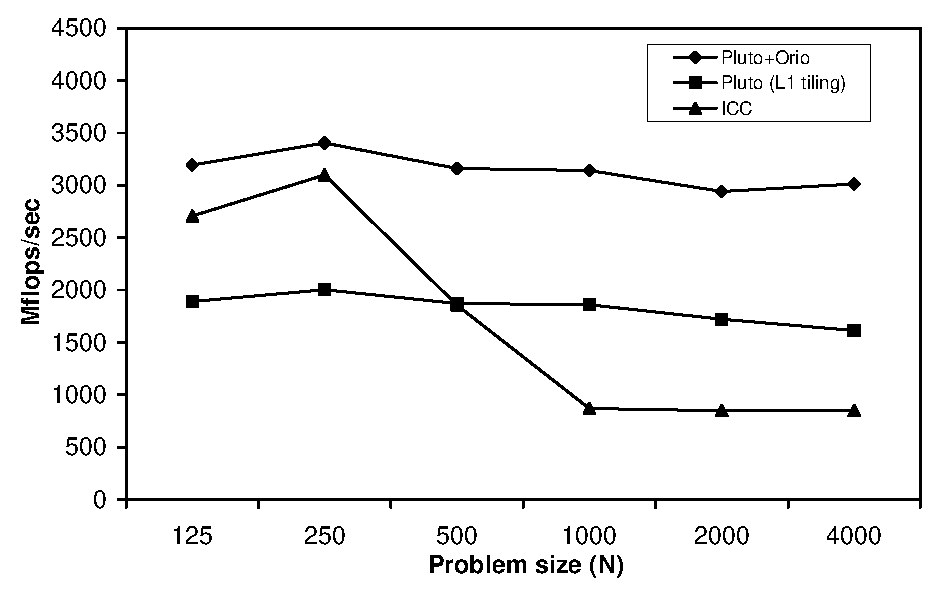
\includegraphics[width=.4\textwidth]{figures/fdtd-2d-cookie/seq.eps} 
  \label{fig:fdtd-2d-cookie-seq} } \subfigure[Parallel (T=500, 
  N=2000)]{ 
  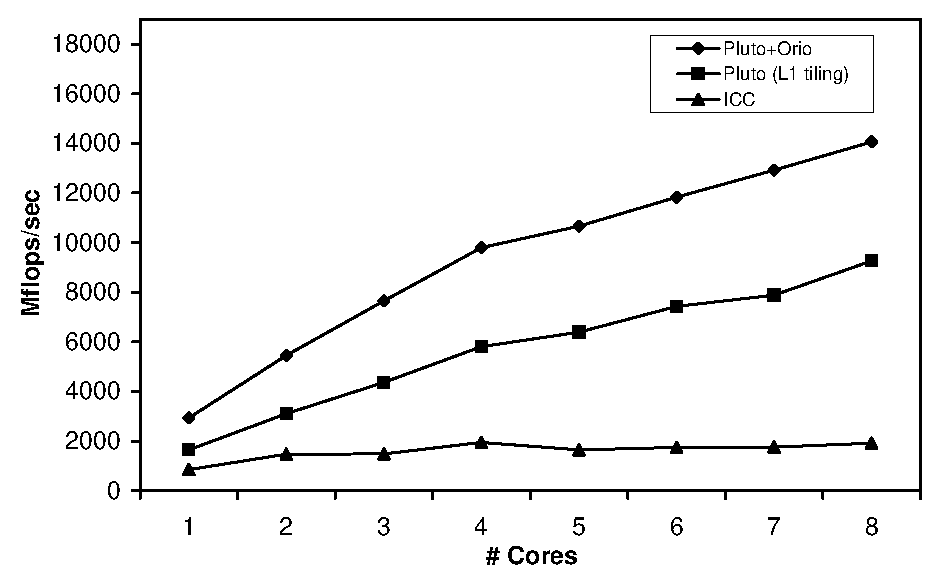
\includegraphics[width=.4\textwidth]{figures/fdtd-2d-cookie/par.eps} 
  \label{fig:fdtd-2d-cookie-par} } 
\end{center}
\vspace{-.2in} 
\caption{2-D FDTD performance on an eight-core Intel Xeon.} 
\label{fig:fdtd-2d-cookie-results} 
%\vspace{-.2in}
\end{figure} 

%%BN: commented out since this needs more explanation (no room in this version)
%It is to be noted that collecting performance results of the PLuTo 
%code with L1 and L2 tilings was not possible because of the large code 
%size of the generated loop nest, which led to an impractically huge 
%compile time. 

%% BN: comment for space
\comment{
\subsubsection{3-D Gauss-Seidel Successive Over-Relaxation Method}  
Figure~\ref{fig:seidel-code} shows the 3-D Gauss-Seidel computation, 
which is sometimes is referred to as
\emph{successive displacement method}, indicating the dependence of the 
iterations on the ordering. If the ordering is
%
%\begin{figure}[ht]
\begin{wrapfigure}{r}{3in}
\vspace{-0.3in}
\begin{center}
\begin{minipage}{3in} 
\scriptsize
\begin{verbatim} 
for (t=0; t<=T-1; t++) 
  for (i=1; i<=N-2; i++) 
    for (j=1; j<=N-2; j++) 
      A[i][j] = (A[i-1][j-1] + A[i-1][j] 
          + A[i-1][j+1] + A[i][j-1] + A[i][j] 
          + A[i][j+1] + A[i+1][j-1] + A[i+1][j] 
          + A[i+1][j+1]) / 9.0; 
\end{verbatim} 
\end{minipage} 
\end{center}
\vspace{-0.2in}
\caption{3-D Gauss-Seidel code} 
\label{fig:seidel-code} 
\vspace{-.1in}
\end{wrapfigure}
%
changed, the components of the new iterations will change as well. 

Figure~\ref{fig:seidel-cookie-seq} contains the sequential performance
results for $T=500$, which show that applying PLuTo's polyhedral tiling on
the original code always delivers performance boosts, which range from 126\%
to 142\%. When using PLuTo, performing two-level tiling (for both L1 and L2
caches) yields 13\% lower performance than performing only L1 tiling. 
This is also reflected in the best sequential code found by Orio, where
one-level tiling (for L1 cache only) is always performed. The sequential
speedup obtained from tuning the PLuTo code with Orio is significant, ranging
from 51\% to 133\%.

\begin{figure} [htb]
\begin{center} 
  \subfigure[Sequential (T=500)]{ 
  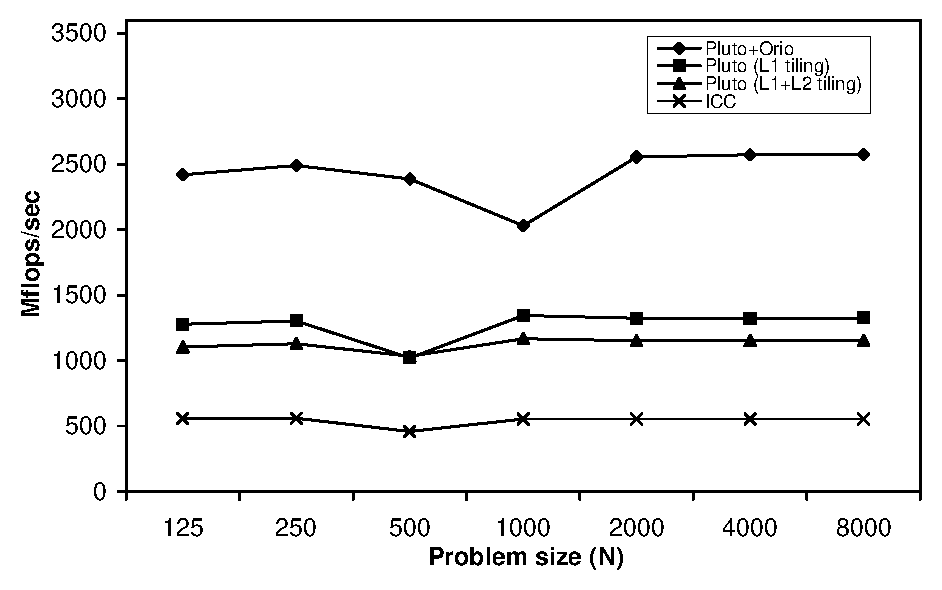
\includegraphics[width=.4\textwidth]{figures/seidel-cookie/seq.eps} 
  \label{fig:seidel-cookie-seq} } \subfigure[Parallel (T=500, 
  N=4000)]{ 
  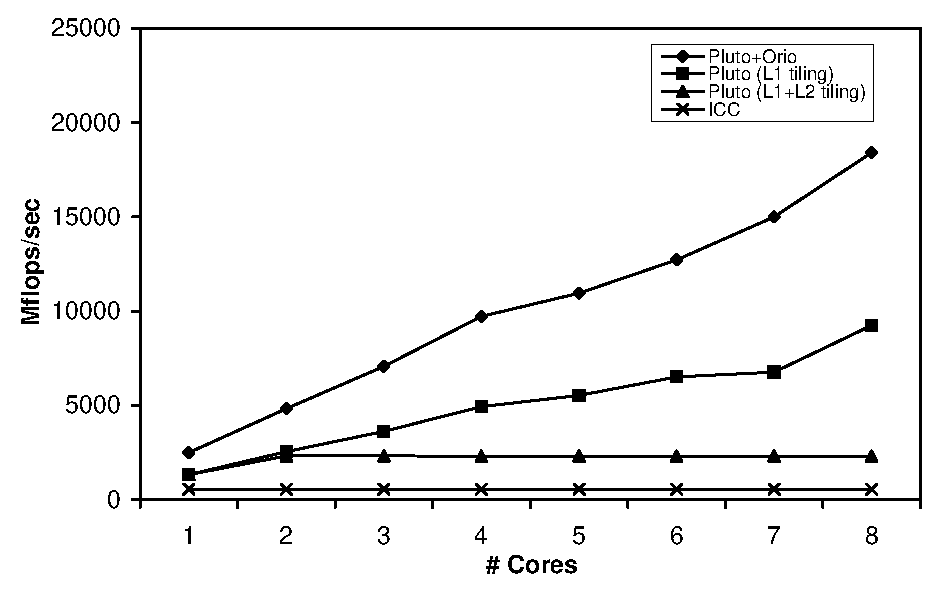
\includegraphics[width=.4\textwidth]{figures/seidel-cookie/par.eps} 
  \label{fig:seidel-cookie-par} } 
\end{center}
\vspace{-.2in} 
\caption{3-D Gauss-Seidel performance on eight-core Intel machine.} 
\label{fig:seidel-cookie-results} 
\vspace{-.1in}
\end{figure} 

The parallel performance results for $T=500$ and $N=4000$ are shown in
Figure~\ref{fig:seidel-cookie-par}. Again we observe that icc failed to
parallelize the code, whereas PLuTo was able to parallelize it and Orio
improved the performance of the one-level tiled PLuTo code further by up to
128\% (and up to 548\% for the two-level tiled PLuTo code). We observed that
tiling over both L1 and L2 can result in worse performance than L1-only
tiling because the number of tiles can be smaller than the number of cores.
%Similar earlier trend also exists
%in these performance results: PLuTo parallelizes the code through its
%polyhedral transformations (i.e., skewing and tiling), while the icc
%compiler alone does not parallelize the loop. Empirical tuning via
%Orio creates up to 122\% speedups over the one-level tiled PLuTo code,
%and up to 548\% speedups over the two-level tiled PLuTo code. Another
%finding is that tiling for both L1 and L2 caches contributes to a poor
%scalability because the number of tiles can be less than the number of
%processors, resulting in underutilization of the available resources.
} % end comment


\subsubsection{LU Factorization}  
 
LU factorization or decomposition is a numerical method for the solution of linear
systems 
%
\begin{wrapfigure}{r}{3in}
\begin{center}
\vspace{-.2in}
\begin{minipage}{2.8in} 
\scriptsize
\begin{verbatim} 
for (k=0; k<=N-1; k++) { 
  for (j=k+1; j<=N-1; j++) 
    A[k][j] /= A[k][k]; 
  for(i=k+1; i<=N-1; i++) 
    for (j=k+1; j<=N-1; j++) 
      A[i][j] -= A[i][k]*A[k][j]; 
} 
\end{verbatim} 
\end{minipage} 
\end{center}
\vspace{-0.2in}
\caption{LU Decomposition code.} 
\label{fig:lu-code} 
\end{wrapfigure}
%
of equations; a simple implementation is shown in Figure~\ref{fig:lu-code}. 

The sequential performance results are shown in
Figure~\ref{fig:lu-cookie-seq}. Similarly to the 2-D FDTD results, the icc-optimized code is more
efficient than the PLuTo-generated codes when the input arrays are small and
fit in the L2 cache. Because of better data locality, however, the
performance of the PLuTo-tiled codes is better than that of the base code as
the input arrays get larger. 
%Again, there are two different codes generated
%by Orio: one for small problem sizes and one for large problem sizes. And
Consequently, Orio employs PLuTo's polyhedral transformations only for large
input sizes prior to applying its own syntactic transformations. 
%Unlike 3-D
%Gauss-Seidel, this time Orio chooses to apply both L1 and L2 tilings when
%generating the best tuned code. 
Compared to the two PLuTo codes, the
Orio-tuned code yields performance improvements ranging between 26\% and 277\%.

The parallel performance results shown in Figure~\ref{fig:lu-cookie-par} were
obtained for $N=4000$. We observe that icc is not able to parallelize the
code, whereas PLuTo achieves higher performance by exploiting multicore
parallelism. Furthermore, both PLuTo-generated codes have comparable
performance, with slightly better scalability exhibited by the single-level tiled
code. Orio further improved the performance of the PLuTo-generated versions
by a factor of 51\% to 120\%.
 
\begin{figure}[htb]
\begin{center} 
  \subfigure[Sequential]{ 
  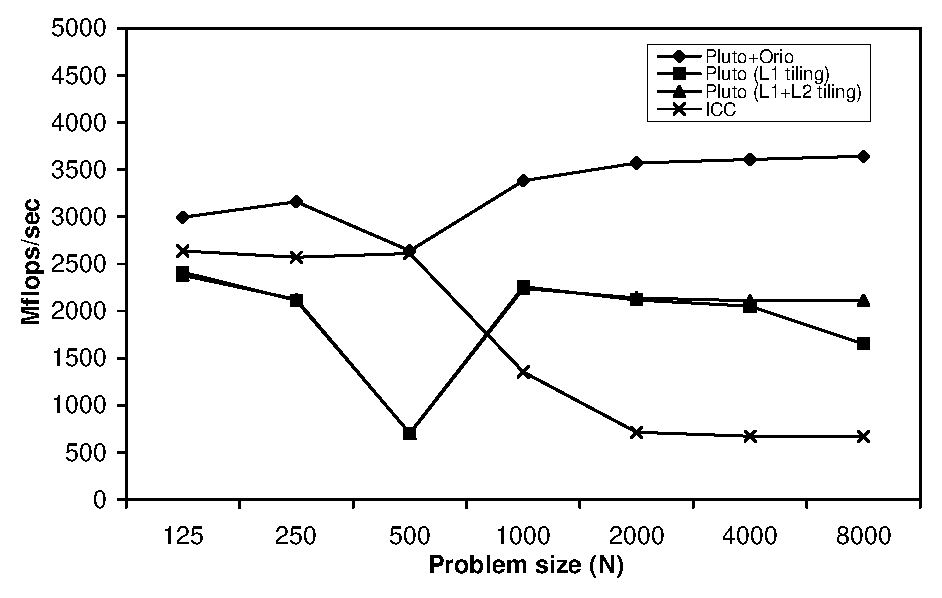
\includegraphics[width=.4\textwidth]{figures/lu-cookie/seq.eps} 
  \label{fig:lu-cookie-seq} } \subfigure[Parallel (N=4000)]{ 
  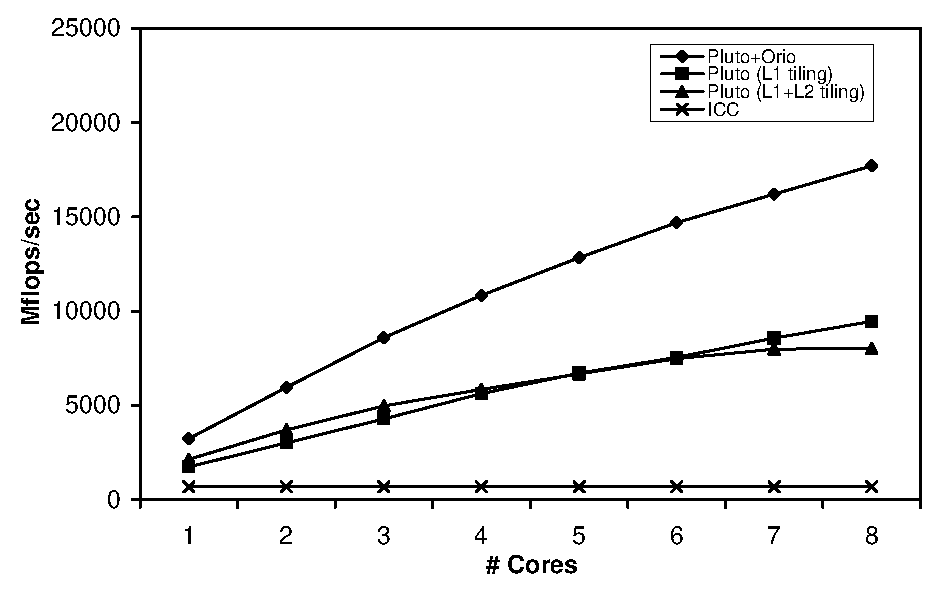
\includegraphics[width=.4\textwidth]{figures/lu-cookie/par.eps} 
  \label{fig:lu-cookie-par} } 
\end{center} 
\vspace{-.2in}
\caption{LU Decomposition performance on eight-core Intel machine.} 
\label{fig:lu-cookie-results} 
\end{figure} 
 
\section{Conclusions and Future Work}
\label{sec:conclusions}

%Future directions:
%- Support for Fortran
%- Supports for various architecture-specific optimizations (e.g., SSE)
%- Automatic tuning for various problem sizes
%- Automatic parallelization for multi-core machines
%- Tuning MPI code (communication minimization)
%- Tuning for GPGPU

%- Build a decision tree that automatically directs to the best tuned code for a given problem size

We have described the design and implementation of Orio, an extensible Python
software system for defining annotation-based performance-improving
transformations. Our experiments with a number of different types of
computations on two different architectures show that Orio can deliver
performance improvements when used alone or in conjunction with other source
transformation tools.

Orio is a new tool under active development; future work includes (but is not
limited to) providing support for annotating and generating Fortran code,
defining new annotation languages and corresponding transformation modules,
e.g., using matrix notation for linear algebra operations, and integration
with other source transformation tools through new optimization modules.

 

\section*{Acknowledgment} 
The authors would like to thank Uday Bondhugula of IBM Research for
many productive discussions and his valuable help with Pluto. This
work was supported in part by the U.S. Dept. of Energy under Contract
DE-AC02-06CH11357, the National Science Foundation through awards
0403342, 0509467, and 0811781, and a State of Ohio Development Fund.

\small
\bibliographystyle{IEEEtran} 
\bibliography{IEEEabrv,paper} 

\end{document}

